\documentclass[12pt,a4paper]{report}
\usepackage[margin=1in]{geometry}
\usepackage[utf8]{inputenc}
\usepackage[T1]{fontenc}
\usepackage{graphicx}
\usepackage{xcolor}
\usepackage{float}
\usepackage{longtable}
\usepackage{array}
\usepackage{booktabs}
\usepackage{hyperref}
\usepackage{enumitem}
\usepackage{setspace}
\usepackage{titlesec}
\usepackage{caption}
\usepackage{ragged2e}
\usepackage{fancyhdr}
\usepackage{tocloft}
\setcounter{tocdepth}{2}
\renewcommand{\contentsname}{Table of Contents}
\renewcommand{\listfigurename}{List of Figures}
\renewcommand{\listtablename}{List of Tables}
\pagestyle{fancy}
\fancyhf{}
\fancyfoot[C]{\thepage}
\renewcommand{\headrulewidth}{0pt}

\hypersetup{colorlinks=true, linkcolor=blue, urlcolor=blue}
\setstretch{1.25}
\setlength{\parindent}{1.2cm}
\setlength{\parskip}{6pt}
\titleformat{\chapter}[display]{\bfseries\centering}{\Large CHAPTER - \thechapter}{1em}{\Huge}
\titleformat{\section}{\Large\bfseries\color{black}}{\thesection}{0.7em}{}
\titleformat{\subsection}{\large\bfseries\color{black}}{\thesubsection}{0.7em}{}
\begin{document}

\pagenumbering{roman}
\begin{titlepage}
\centering
\vspace*{0.4cm}
{\Large\bfseries AI-Driven Real-Time Interview Simulation and Recruitment System\par}
\vspace{1.2cm}
{\large A project report submitted in partial fulfillment of the requirements\par}
{\large for the award of the degree of\par}
\vspace{0.5cm}
{\Large\bfseries MASTER OF COMPUTER APPLICATIONS\par}
\vspace{1.0cm}
{\large\bfseries By\par}
\vspace{0.25cm}
{\Large\bfseries NAGA SUBRAHMANYAM\par}
{\large\bfseries 23VV1F0016\par}
\vspace{1.0cm}
{\large Under the Esteemed Guidance of\par}
{\large\bfseries Project Guide\par}
\vfill
{\large\bfseries DEPARTMENT OF INFORMATION TECHNOLOGY\par}
\vspace{0.25cm}
{\large\bfseries JNTUGV College of Engineering Vizianagaram (Autonomous)\par}
{\large Jawaharlal Nehru Technological University, Gurajada Vizianagaram\par}
{\large Dwarapudi, Vizianagaram - 535003, Andhra Pradesh, India\par}
\vspace{0.5cm}
{\large 2025--2026\par}
\end{titlepage}

\chapter*{CERTIFICATE}
\addcontentsline{toc}{chapter}{CERTIFICATE}
\justifying
This is to certify that the project report entitled ``AI-Driven Real-Time Interview Simulation and Recruitment System'' submitted by NAGA SUBRAHMANYAM bearing registration number 23VV1F0016 is prepared in partial fulfillment for the award of the degree of Master of Computer Applications. The work presented in this report was carried out as a project study on a full-stack interview simulation and recruitment platform using modern web technologies, artificial intelligence services, and real-time communication components.

The contents of this report describe the design, implementation, testing, and analysis of the developed system. The results embodied in this project have not been submitted to any other university or institute for the award of any degree or diploma.

\vspace{1.8cm}
\noindent\begin{tabular}{p{0.45\textwidth}p{0.45\textwidth}}
Signature of the Supervisor & Signature of the Head of the Department\\[1.6cm]
Project Guide & Head of the Department\\[1.4cm]
\multicolumn{2}{c}{External Signature}
\end{tabular}

\clearpage
\chapter*{DECLARATION}
\addcontentsline{toc}{chapter}{DECLARATION}
\justifying
I, NAGA SUBRAHMANYAM with Reg. No: 23VV1F0016, declare that this submission represents my own project work and report writing. Where external technologies, documentation, or standard references have been used, they are acknowledged in the references section. I also declare that I have not misrepresented or falsified any project implementation, data, or result described in this report.

\vspace{1.5cm}
\noindent Date:\\
Place:

\vspace{1.5cm}
\begin{flushright}
(Signature)\\
NAGA SUBRAHMANYAM\\
23VV1F0016
\end{flushright}

\clearpage
\chapter*{ACKNOWLEDGEMENT}
\addcontentsline{toc}{chapter}{ACKNOWLEDGEMENT}
\justifying
I express my sincere gratitude to my project guide and faculty members for their guidance, encouragement, and support throughout the completion of this project. Their suggestions helped in refining the problem statement, improving the design, and presenting the implementation in an organized academic form.

I also thank the Department of Information Technology and the institution for providing the academic environment required to complete this work. The project required knowledge of web development, databases, artificial intelligence, real-time communication, and software testing, and the learning support provided by the department was valuable.

Finally, I thank my family, friends, and peers for their motivation and feedback during the development and documentation of the AI-driven interview simulation system.

\clearpage
\chapter*{ABSTRACT}
\addcontentsline{toc}{chapter}{ABSTRACT}
\justifying
Interview preparation and recruitment evaluation are increasingly dependent on digital platforms, yet many existing systems handle only isolated tasks such as video calling, coding practice, or resume screening. This project presents an AI-driven real-time interview simulation and recruitment system that combines mock interviews, coding interviews, peer practice, recruiter-led sessions, AI coaching, learning roadmaps, resume handling, and performance reporting inside one browser-based application.

The system is developed using React, Vite, and Tailwind CSS for the frontend, Node.js and Express for backend APIs, MongoDB and Mongoose for persistence, Socket.IO and WebRTC for real-time collaboration, Web Speech API for speech input, browser camera analysis for monitoring, and Gemini AI services for question generation, coaching, and evaluation support. The platform supports authentication with email verification, live AI interviews, LeetCode-style coding practice, competitive coding battle rooms, peer mock interview requests, recruiter interview rooms, AI-generated reports, and personalized learning roadmaps.

The project aims to reduce fragmented interview preparation by offering a unified workflow that records answers, evaluates responses, tracks progress, and provides actionable feedback. Results show that the application can provide a structured interview experience with automated question flow, real-time user interaction, and stored performance history. The system is suitable for students, job seekers, training institutions, and recruiters who need a scalable interview preparation and assessment environment.

\clearpage
\chapter*{ABBREVIATIONS}
\addcontentsline{toc}{chapter}{ABBREVIATIONS}
\begin{longtable}{|>{\raggedright\arraybackslash}p{0.28\textwidth}|>{\raggedright\arraybackslash}p{0.62\textwidth}|}
\hline
\textbf{Abbreviation} & \textbf{Meaning}\\
\hline
AI & Artificial Intelligence\\\hline
API & Application Programming Interface\\\hline
JWT & JSON Web Token\\\hline
MERN & MongoDB, Express.js, React, Node.js\\\hline
OTP & One-Time Password\\\hline
REST & Representational State Transfer\\\hline
STT & Speech-to-Text\\\hline
TTS & Text-to-Speech\\\hline
UI & User Interface\\\hline
WebRTC & Web Real-Time Communication\\\hline
\end{longtable}

\clearpage
\tableofcontents
\clearpage
\listoffigures
\clearpage
\listoftables
\clearpage
\pagenumbering{arabic}
\chapter{INTRODUCTION}

\section{Introduction to Interview Simulation}

Introduction to Interview Simulation is a central part of the proposed AI-driven interview simulation system because it connects the user-facing experience with measurable recruitment outcomes. In this project, the feature is implemented as part of a browser-based platform where candidates can prepare, recruiters can evaluate, and peers can collaborate without switching between separate tools.


The implementation uses React, Vite, and Tailwind CSS on the client side to keep the user interface responsive and consistent. The backend uses Node.js and Express to expose secure REST APIs, while MongoDB stores users, interview sessions, responses, reports, roadmaps, rooms, and activity history. This separation keeps presentation logic, business logic, and data persistence understandable for maintenance and review.


In the context of realistic interview preparation, the system captures structured inputs from the user and converts them into useful interview actions. These actions include authentication, interview configuration, camera and microphone activation, AI question delivery, answer submission, code execution, peer connection, recruiter scoring, and report generation depending on the selected module.


The major modules involved are authentication, setup, live interview room, camera monitoring, speech recognition, reports. Their interaction is designed to reduce manual effort while preserving the natural flow of an interview. AI services assist with question generation and coaching, but the application still keeps final data storage, permissions, and workflow control inside the backend server.


The design also considers practical constraints such as browser permissions, network reliability, free deployment limitations, and API quota limits. Therefore, fallback behavior, clear error messages, and modular routing are important engineering decisions in the project. These decisions make the platform suitable for academic demonstration as well as a foundation for future production improvements.


From a software engineering point of view, introduction to interview simulation is not treated as an isolated screen. It is connected to routing, protected access, backend validation, database persistence, and user feedback. This approach prevents a common problem in student projects where screens look complete but do not share consistent state or saved records.


The project follows a practical full-stack pattern in which the client sends only the required data to the server and the server performs sensitive operations such as authentication, AI API calls, and database writes. This keeps credentials and API keys away from the browser and provides one controlled place to apply error handling, logging, and validation.


For review and testing, this part of the system can be demonstrated through a clear sequence of actions: open the module, submit valid input, observe the server response, inspect stored history, and verify the final user-facing output. This sequence makes the implementation easier to explain during viva and final evaluation because each visible screen maps to a backend responsibility.


The design also improves future maintainability. Since routes, models, and pages are organized by feature, new capabilities such as advanced analytics, stronger coding judge support, multi-provider AI, institution dashboards, or recruiter comparison reports can be added without rewriting the whole application.


\section{Artificial Intelligence in Recruitment}

Artificial Intelligence in Recruitment is a central part of the proposed AI-driven interview simulation system because it connects the user-facing experience with measurable recruitment outcomes. In this project, the feature is implemented as part of a browser-based platform where candidates can prepare, recruiters can evaluate, and peers can collaborate without switching between separate tools.


The implementation uses React, Vite, and Tailwind CSS on the client side to keep the user interface responsive and consistent. The backend uses Node.js and Express to expose secure REST APIs, while MongoDB stores users, interview sessions, responses, reports, roadmaps, rooms, and activity history. This separation keeps presentation logic, business logic, and data persistence understandable for maintenance and review.


In the context of AI-assisted screening and feedback, the system captures structured inputs from the user and converts them into useful interview actions. These actions include authentication, interview configuration, camera and microphone activation, AI question delivery, answer submission, code execution, peer connection, recruiter scoring, and report generation depending on the selected module.


The major modules involved are Gemini services, prompt generation, answer evaluation, AI coach, learning roadmaps. Their interaction is designed to reduce manual effort while preserving the natural flow of an interview. AI services assist with question generation and coaching, but the application still keeps final data storage, permissions, and workflow control inside the backend server.


The design also considers practical constraints such as browser permissions, network reliability, free deployment limitations, and API quota limits. Therefore, fallback behavior, clear error messages, and modular routing are important engineering decisions in the project. These decisions make the platform suitable for academic demonstration as well as a foundation for future production improvements.


From a software engineering point of view, artificial intelligence in recruitment is not treated as an isolated screen. It is connected to routing, protected access, backend validation, database persistence, and user feedback. This approach prevents a common problem in student projects where screens look complete but do not share consistent state or saved records.


The project follows a practical full-stack pattern in which the client sends only the required data to the server and the server performs sensitive operations such as authentication, AI API calls, and database writes. This keeps credentials and API keys away from the browser and provides one controlled place to apply error handling, logging, and validation.


For review and testing, this part of the system can be demonstrated through a clear sequence of actions: open the module, submit valid input, observe the server response, inspect stored history, and verify the final user-facing output. This sequence makes the implementation easier to explain during viva and final evaluation because each visible screen maps to a backend responsibility.


The design also improves future maintainability. Since routes, models, and pages are organized by feature, new capabilities such as advanced analytics, stronger coding judge support, multi-provider AI, institution dashboards, or recruiter comparison reports can be added without rewriting the whole application.


\section{Problem Statement}

Problem Statement is a central part of the proposed AI-driven interview simulation system because it connects the user-facing experience with measurable recruitment outcomes. In this project, the feature is implemented as part of a browser-based platform where candidates can prepare, recruiters can evaluate, and peers can collaborate without switching between separate tools.


The implementation uses React, Vite, and Tailwind CSS on the client side to keep the user interface responsive and consistent. The backend uses Node.js and Express to expose secure REST APIs, while MongoDB stores users, interview sessions, responses, reports, roadmaps, rooms, and activity history. This separation keeps presentation logic, business logic, and data persistence understandable for maintenance and review.


In the context of fragmented preparation and subjective interviews, the system captures structured inputs from the user and converts them into useful interview actions. These actions include authentication, interview configuration, camera and microphone activation, AI question delivery, answer submission, code execution, peer connection, recruiter scoring, and report generation depending on the selected module.


The major modules involved are mock interviews, coding practice, peer rooms, recruiter portal, analytics. Their interaction is designed to reduce manual effort while preserving the natural flow of an interview. AI services assist with question generation and coaching, but the application still keeps final data storage, permissions, and workflow control inside the backend server.


The design also considers practical constraints such as browser permissions, network reliability, free deployment limitations, and API quota limits. Therefore, fallback behavior, clear error messages, and modular routing are important engineering decisions in the project. These decisions make the platform suitable for academic demonstration as well as a foundation for future production improvements.


From a software engineering point of view, problem statement is not treated as an isolated screen. It is connected to routing, protected access, backend validation, database persistence, and user feedback. This approach prevents a common problem in student projects where screens look complete but do not share consistent state or saved records.


The project follows a practical full-stack pattern in which the client sends only the required data to the server and the server performs sensitive operations such as authentication, AI API calls, and database writes. This keeps credentials and API keys away from the browser and provides one controlled place to apply error handling, logging, and validation.


For review and testing, this part of the system can be demonstrated through a clear sequence of actions: open the module, submit valid input, observe the server response, inspect stored history, and verify the final user-facing output. This sequence makes the implementation easier to explain during viva and final evaluation because each visible screen maps to a backend responsibility.


The design also improves future maintainability. Since routes, models, and pages are organized by feature, new capabilities such as advanced analytics, stronger coding judge support, multi-provider AI, institution dashboards, or recruiter comparison reports can be added without rewriting the whole application.


\section{Objectives of the Project}

Objectives of the Project is a central part of the proposed AI-driven interview simulation system because it connects the user-facing experience with measurable recruitment outcomes. In this project, the feature is implemented as part of a browser-based platform where candidates can prepare, recruiters can evaluate, and peers can collaborate without switching between separate tools.


The implementation uses React, Vite, and Tailwind CSS on the client side to keep the user interface responsive and consistent. The backend uses Node.js and Express to expose secure REST APIs, while MongoDB stores users, interview sessions, responses, reports, roadmaps, rooms, and activity history. This separation keeps presentation logic, business logic, and data persistence understandable for maintenance and review.


In the context of clear measurable project goals, the system captures structured inputs from the user and converts them into useful interview actions. These actions include authentication, interview configuration, camera and microphone activation, AI question delivery, answer submission, code execution, peer connection, recruiter scoring, and report generation depending on the selected module.


The major modules involved are AI interview module, coding environment, peer collaboration, recruiter workflow, dashboard reports. Their interaction is designed to reduce manual effort while preserving the natural flow of an interview. AI services assist with question generation and coaching, but the application still keeps final data storage, permissions, and workflow control inside the backend server.


The design also considers practical constraints such as browser permissions, network reliability, free deployment limitations, and API quota limits. Therefore, fallback behavior, clear error messages, and modular routing are important engineering decisions in the project. These decisions make the platform suitable for academic demonstration as well as a foundation for future production improvements.


From a software engineering point of view, objectives of the project is not treated as an isolated screen. It is connected to routing, protected access, backend validation, database persistence, and user feedback. This approach prevents a common problem in student projects where screens look complete but do not share consistent state or saved records.


The project follows a practical full-stack pattern in which the client sends only the required data to the server and the server performs sensitive operations such as authentication, AI API calls, and database writes. This keeps credentials and API keys away from the browser and provides one controlled place to apply error handling, logging, and validation.


For review and testing, this part of the system can be demonstrated through a clear sequence of actions: open the module, submit valid input, observe the server response, inspect stored history, and verify the final user-facing output. This sequence makes the implementation easier to explain during viva and final evaluation because each visible screen maps to a backend responsibility.


The design also improves future maintainability. Since routes, models, and pages are organized by feature, new capabilities such as advanced analytics, stronger coding judge support, multi-provider AI, institution dashboards, or recruiter comparison reports can be added without rewriting the whole application.


\begin{itemize}
\item Provide a single browser-based platform for interview preparation and recruitment evaluation.
\end{itemize}

\begin{itemize}
\item Generate role-based and topic-based interview questions using AI assistance.
\end{itemize}

\begin{itemize}
\item Capture spoken or typed answers and store structured response history.
\end{itemize}

\begin{itemize}
\item Support coding practice and competitive coding battle flows.
\end{itemize}

\begin{itemize}
\item Enable peer mock interviews and recruiter live interview rooms.
\end{itemize}

\begin{itemize}
\item Provide reports, learning roadmaps, and AI coaching for continuous improvement.
\end{itemize}

\section{Scope of the Project}

Scope of the Project is a central part of the proposed AI-driven interview simulation system because it connects the user-facing experience with measurable recruitment outcomes. In this project, the feature is implemented as part of a browser-based platform where candidates can prepare, recruiters can evaluate, and peers can collaborate without switching between separate tools.


The implementation uses React, Vite, and Tailwind CSS on the client side to keep the user interface responsive and consistent. The backend uses Node.js and Express to expose secure REST APIs, while MongoDB stores users, interview sessions, responses, reports, roadmaps, rooms, and activity history. This separation keeps presentation logic, business logic, and data persistence understandable for maintenance and review.


In the context of boundaries of the implemented system, the system captures structured inputs from the user and converts them into useful interview actions. These actions include authentication, interview configuration, camera and microphone activation, AI question delivery, answer submission, code execution, peer connection, recruiter scoring, and report generation depending on the selected module.


The major modules involved are React client, Express API, MongoDB database, real-time rooms, AI integration. Their interaction is designed to reduce manual effort while preserving the natural flow of an interview. AI services assist with question generation and coaching, but the application still keeps final data storage, permissions, and workflow control inside the backend server.


The design also considers practical constraints such as browser permissions, network reliability, free deployment limitations, and API quota limits. Therefore, fallback behavior, clear error messages, and modular routing are important engineering decisions in the project. These decisions make the platform suitable for academic demonstration as well as a foundation for future production improvements.


From a software engineering point of view, scope of the project is not treated as an isolated screen. It is connected to routing, protected access, backend validation, database persistence, and user feedback. This approach prevents a common problem in student projects where screens look complete but do not share consistent state or saved records.


The project follows a practical full-stack pattern in which the client sends only the required data to the server and the server performs sensitive operations such as authentication, AI API calls, and database writes. This keeps credentials and API keys away from the browser and provides one controlled place to apply error handling, logging, and validation.


For review and testing, this part of the system can be demonstrated through a clear sequence of actions: open the module, submit valid input, observe the server response, inspect stored history, and verify the final user-facing output. This sequence makes the implementation easier to explain during viva and final evaluation because each visible screen maps to a backend responsibility.


The design also improves future maintainability. Since routes, models, and pages are organized by feature, new capabilities such as advanced analytics, stronger coding judge support, multi-provider AI, institution dashboards, or recruiter comparison reports can be added without rewriting the whole application.


\section{Organization of the Report}

Organization of the Report is a central part of the proposed AI-driven interview simulation system because it connects the user-facing experience with measurable recruitment outcomes. In this project, the feature is implemented as part of a browser-based platform where candidates can prepare, recruiters can evaluate, and peers can collaborate without switching between separate tools.


The implementation uses React, Vite, and Tailwind CSS on the client side to keep the user interface responsive and consistent. The backend uses Node.js and Express to expose secure REST APIs, while MongoDB stores users, interview sessions, responses, reports, roadmaps, rooms, and activity history. This separation keeps presentation logic, business logic, and data persistence understandable for maintenance and review.


In the context of report navigation, the system captures structured inputs from the user and converts them into useful interview actions. These actions include authentication, interview configuration, camera and microphone activation, AI question delivery, answer submission, code execution, peer connection, recruiter scoring, and report generation depending on the selected module.


The major modules involved are requirements, design, implementation, results, conclusion, appendices. Their interaction is designed to reduce manual effort while preserving the natural flow of an interview. AI services assist with question generation and coaching, but the application still keeps final data storage, permissions, and workflow control inside the backend server.


The design also considers practical constraints such as browser permissions, network reliability, free deployment limitations, and API quota limits. Therefore, fallback behavior, clear error messages, and modular routing are important engineering decisions in the project. These decisions make the platform suitable for academic demonstration as well as a foundation for future production improvements.


From a software engineering point of view, organization of the report is not treated as an isolated screen. It is connected to routing, protected access, backend validation, database persistence, and user feedback. This approach prevents a common problem in student projects where screens look complete but do not share consistent state or saved records.


The project follows a practical full-stack pattern in which the client sends only the required data to the server and the server performs sensitive operations such as authentication, AI API calls, and database writes. This keeps credentials and API keys away from the browser and provides one controlled place to apply error handling, logging, and validation.


For review and testing, this part of the system can be demonstrated through a clear sequence of actions: open the module, submit valid input, observe the server response, inspect stored history, and verify the final user-facing output. This sequence makes the implementation easier to explain during viva and final evaluation because each visible screen maps to a backend responsibility.


The design also improves future maintainability. Since routes, models, and pages are organized by feature, new capabilities such as advanced analytics, stronger coding judge support, multi-provider AI, institution dashboards, or recruiter comparison reports can be added without rewriting the whole application.


\begin{figure}[H]
\centering
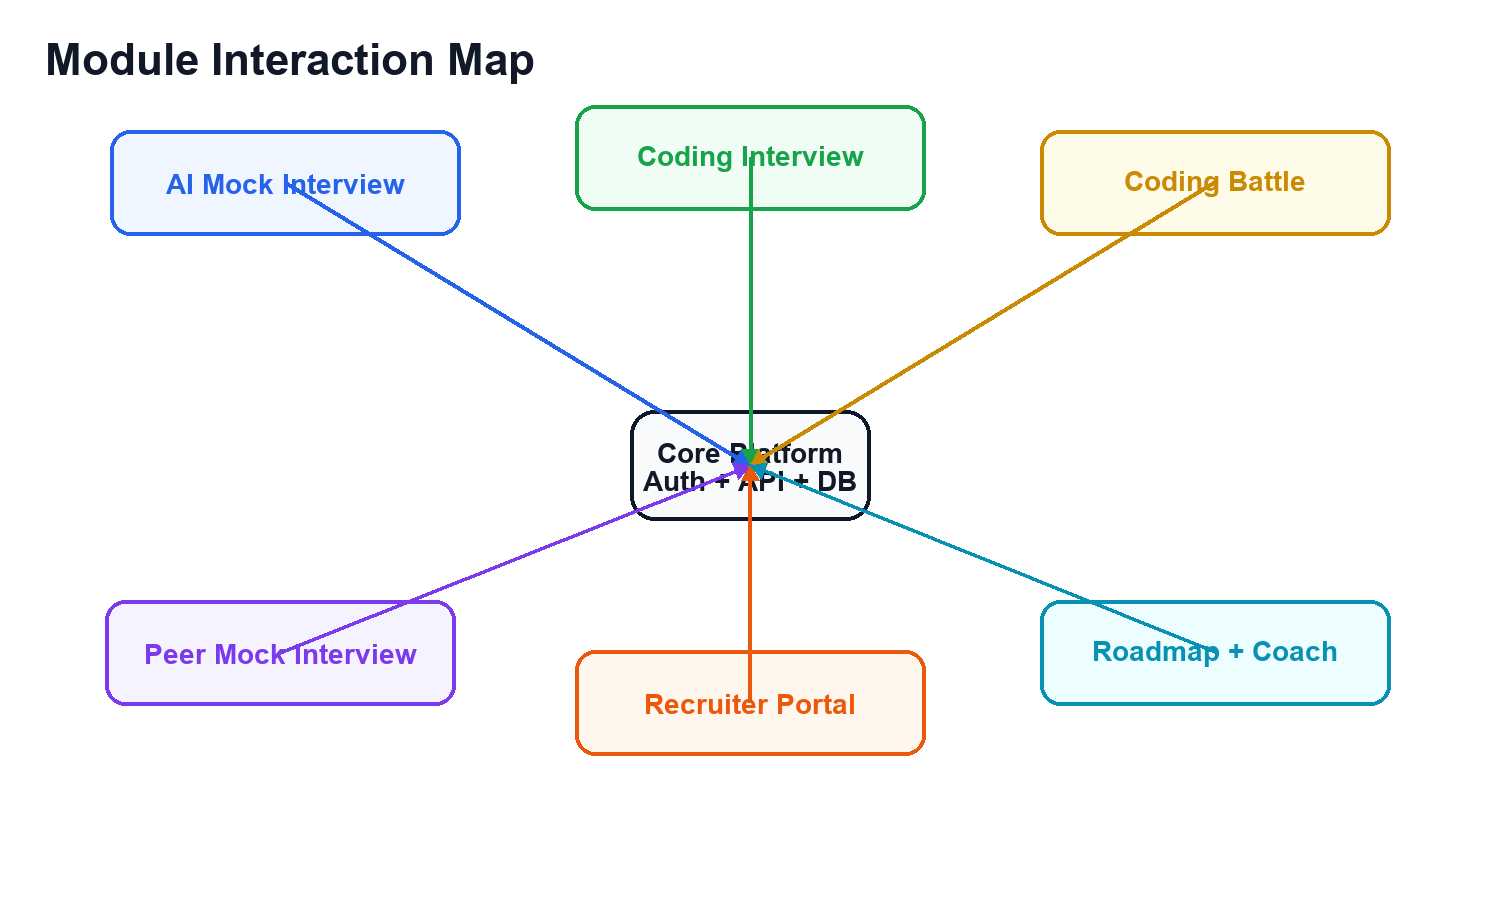
\includegraphics[width=0.95\textwidth]{AI_Driven_Interview_Simulation_Final_Report_assets/figure_01.png}
\caption{Overall module interaction map of the project}
\end{figure}


\chapter{LITERATURE SURVEY}

\section{Existing Interview Platforms}

Existing Interview Platforms is a central part of the proposed AI-driven interview simulation system because it connects the user-facing experience with measurable recruitment outcomes. In this project, the feature is implemented as part of a browser-based platform where candidates can prepare, recruiters can evaluate, and peers can collaborate without switching between separate tools.


The implementation uses React, Vite, and Tailwind CSS on the client side to keep the user interface responsive and consistent. The backend uses Node.js and Express to expose secure REST APIs, while MongoDB stores users, interview sessions, responses, reports, roadmaps, rooms, and activity history. This separation keeps presentation logic, business logic, and data persistence understandable for maintenance and review.


In the context of comparison with interview practice tools, the system captures structured inputs from the user and converts them into useful interview actions. These actions include authentication, interview configuration, camera and microphone activation, AI question delivery, answer submission, code execution, peer connection, recruiter scoring, and report generation depending on the selected module.


The major modules involved are video meeting apps, coding judges, resume tools, LMS-based practice systems. Their interaction is designed to reduce manual effort while preserving the natural flow of an interview. AI services assist with question generation and coaching, but the application still keeps final data storage, permissions, and workflow control inside the backend server.


The design also considers practical constraints such as browser permissions, network reliability, free deployment limitations, and API quota limits. Therefore, fallback behavior, clear error messages, and modular routing are important engineering decisions in the project. These decisions make the platform suitable for academic demonstration as well as a foundation for future production improvements.


From a software engineering point of view, existing interview platforms is not treated as an isolated screen. It is connected to routing, protected access, backend validation, database persistence, and user feedback. This approach prevents a common problem in student projects where screens look complete but do not share consistent state or saved records.


The project follows a practical full-stack pattern in which the client sends only the required data to the server and the server performs sensitive operations such as authentication, AI API calls, and database writes. This keeps credentials and API keys away from the browser and provides one controlled place to apply error handling, logging, and validation.


For review and testing, this part of the system can be demonstrated through a clear sequence of actions: open the module, submit valid input, observe the server response, inspect stored history, and verify the final user-facing output. This sequence makes the implementation easier to explain during viva and final evaluation because each visible screen maps to a backend responsibility.


The design also improves future maintainability. Since routes, models, and pages are organized by feature, new capabilities such as advanced analytics, stronger coding judge support, multi-provider AI, institution dashboards, or recruiter comparison reports can be added without rewriting the whole application.


\section{AI-Based Recruitment Systems}

AI-Based Recruitment Systems is a central part of the proposed AI-driven interview simulation system because it connects the user-facing experience with measurable recruitment outcomes. In this project, the feature is implemented as part of a browser-based platform where candidates can prepare, recruiters can evaluate, and peers can collaborate without switching between separate tools.


The implementation uses React, Vite, and Tailwind CSS on the client side to keep the user interface responsive and consistent. The backend uses Node.js and Express to expose secure REST APIs, while MongoDB stores users, interview sessions, responses, reports, roadmaps, rooms, and activity history. This separation keeps presentation logic, business logic, and data persistence understandable for maintenance and review.


In the context of AI use in recruitment pipelines, the system captures structured inputs from the user and converts them into useful interview actions. These actions include authentication, interview configuration, camera and microphone activation, AI question delivery, answer submission, code execution, peer connection, recruiter scoring, and report generation depending on the selected module.


The major modules involved are LLM question generation, resume parsing, scoring rubrics, structured feedback. Their interaction is designed to reduce manual effort while preserving the natural flow of an interview. AI services assist with question generation and coaching, but the application still keeps final data storage, permissions, and workflow control inside the backend server.


The design also considers practical constraints such as browser permissions, network reliability, free deployment limitations, and API quota limits. Therefore, fallback behavior, clear error messages, and modular routing are important engineering decisions in the project. These decisions make the platform suitable for academic demonstration as well as a foundation for future production improvements.


From a software engineering point of view, ai-based recruitment systems is not treated as an isolated screen. It is connected to routing, protected access, backend validation, database persistence, and user feedback. This approach prevents a common problem in student projects where screens look complete but do not share consistent state or saved records.


The project follows a practical full-stack pattern in which the client sends only the required data to the server and the server performs sensitive operations such as authentication, AI API calls, and database writes. This keeps credentials and API keys away from the browser and provides one controlled place to apply error handling, logging, and validation.


For review and testing, this part of the system can be demonstrated through a clear sequence of actions: open the module, submit valid input, observe the server response, inspect stored history, and verify the final user-facing output. This sequence makes the implementation easier to explain during viva and final evaluation because each visible screen maps to a backend responsibility.


The design also improves future maintainability. Since routes, models, and pages are organized by feature, new capabilities such as advanced analytics, stronger coding judge support, multi-provider AI, institution dashboards, or recruiter comparison reports can be added without rewriting the whole application.


\section{Research Gap}

Research Gap is a central part of the proposed AI-driven interview simulation system because it connects the user-facing experience with measurable recruitment outcomes. In this project, the feature is implemented as part of a browser-based platform where candidates can prepare, recruiters can evaluate, and peers can collaborate without switching between separate tools.


The implementation uses React, Vite, and Tailwind CSS on the client side to keep the user interface responsive and consistent. The backend uses Node.js and Express to expose secure REST APIs, while MongoDB stores users, interview sessions, responses, reports, roadmaps, rooms, and activity history. This separation keeps presentation logic, business logic, and data persistence understandable for maintenance and review.


In the context of limitations of current systems, the system captures structured inputs from the user and converts them into useful interview actions. These actions include authentication, interview configuration, camera and microphone activation, AI question delivery, answer submission, code execution, peer connection, recruiter scoring, and report generation depending on the selected module.


The major modules involved are fragmented workflows, lack of real-time analysis, limited peer matching, missing recruiter integration. Their interaction is designed to reduce manual effort while preserving the natural flow of an interview. AI services assist with question generation and coaching, but the application still keeps final data storage, permissions, and workflow control inside the backend server.


The design also considers practical constraints such as browser permissions, network reliability, free deployment limitations, and API quota limits. Therefore, fallback behavior, clear error messages, and modular routing are important engineering decisions in the project. These decisions make the platform suitable for academic demonstration as well as a foundation for future production improvements.


From a software engineering point of view, research gap is not treated as an isolated screen. It is connected to routing, protected access, backend validation, database persistence, and user feedback. This approach prevents a common problem in student projects where screens look complete but do not share consistent state or saved records.


The project follows a practical full-stack pattern in which the client sends only the required data to the server and the server performs sensitive operations such as authentication, AI API calls, and database writes. This keeps credentials and API keys away from the browser and provides one controlled place to apply error handling, logging, and validation.


For review and testing, this part of the system can be demonstrated through a clear sequence of actions: open the module, submit valid input, observe the server response, inspect stored history, and verify the final user-facing output. This sequence makes the implementation easier to explain during viva and final evaluation because each visible screen maps to a backend responsibility.


The design also improves future maintainability. Since routes, models, and pages are organized by feature, new capabilities such as advanced analytics, stronger coding judge support, multi-provider AI, institution dashboards, or recruiter comparison reports can be added without rewriting the whole application.


\section{Proposed Solution}

Proposed Solution is a central part of the proposed AI-driven interview simulation system because it connects the user-facing experience with measurable recruitment outcomes. In this project, the feature is implemented as part of a browser-based platform where candidates can prepare, recruiters can evaluate, and peers can collaborate without switching between separate tools.


The implementation uses React, Vite, and Tailwind CSS on the client side to keep the user interface responsive and consistent. The backend uses Node.js and Express to expose secure REST APIs, while MongoDB stores users, interview sessions, responses, reports, roadmaps, rooms, and activity history. This separation keeps presentation logic, business logic, and data persistence understandable for maintenance and review.


In the context of unified web platform, the system captures structured inputs from the user and converts them into useful interview actions. These actions include authentication, interview configuration, camera and microphone activation, AI question delivery, answer submission, code execution, peer connection, recruiter scoring, and report generation depending on the selected module.


The major modules involved are AI interview, coding battle, peer mock interview, recruiter portal, career roadmap, AI coach. Their interaction is designed to reduce manual effort while preserving the natural flow of an interview. AI services assist with question generation and coaching, but the application still keeps final data storage, permissions, and workflow control inside the backend server.


The design also considers practical constraints such as browser permissions, network reliability, free deployment limitations, and API quota limits. Therefore, fallback behavior, clear error messages, and modular routing are important engineering decisions in the project. These decisions make the platform suitable for academic demonstration as well as a foundation for future production improvements.


From a software engineering point of view, proposed solution is not treated as an isolated screen. It is connected to routing, protected access, backend validation, database persistence, and user feedback. This approach prevents a common problem in student projects where screens look complete but do not share consistent state or saved records.


The project follows a practical full-stack pattern in which the client sends only the required data to the server and the server performs sensitive operations such as authentication, AI API calls, and database writes. This keeps credentials and API keys away from the browser and provides one controlled place to apply error handling, logging, and validation.


For review and testing, this part of the system can be demonstrated through a clear sequence of actions: open the module, submit valid input, observe the server response, inspect stored history, and verify the final user-facing output. This sequence makes the implementation easier to explain during viva and final evaluation because each visible screen maps to a backend responsibility.


The design also improves future maintainability. Since routes, models, and pages are organized by feature, new capabilities such as advanced analytics, stronger coding judge support, multi-provider AI, institution dashboards, or recruiter comparison reports can be added without rewriting the whole application.


\begin{longtable}{|>{\raggedright\arraybackslash}p{0.31\textwidth}|>{\raggedright\arraybackslash}p{0.31\textwidth}|>{\raggedright\arraybackslash}p{0.31\textwidth}|}
\hline
Traditional System & Limitation & Proposed System Improvement \\
\hline
\endfirsthead
\hline
Traditional System & Limitation & Proposed System Improvement \\
\hline
\endhead
Separate video and coding tools & Data is fragmented and difficult to evaluate & Integrated interview room with camera, microphone, chat, code, and reports \\
\hline
Manual feedback & Slow and subjective & AI-assisted structured evaluation and stored report history \\
\hline
Static coding practice & No interview pressure & Coding interview and coding battle with timed flow \\
\hline
No peer discovery & Students cannot easily practice together & Peer mock interview requests and shared rooms \\
\hline
Recruiter notes only & Hard to standardize scoring & Recruiter portal with scoring and room history \\
\hline
\end{longtable}

\chapter{REQUIREMENTS}

\section{Software Requirements}

Software Requirements is a central part of the proposed AI-driven interview simulation system because it connects the user-facing experience with measurable recruitment outcomes. In this project, the feature is implemented as part of a browser-based platform where candidates can prepare, recruiters can evaluate, and peers can collaborate without switching between separate tools.


The implementation uses React, Vite, and Tailwind CSS on the client side to keep the user interface responsive and consistent. The backend uses Node.js and Express to expose secure REST APIs, while MongoDB stores users, interview sessions, responses, reports, roadmaps, rooms, and activity history. This separation keeps presentation logic, business logic, and data persistence understandable for maintenance and review.


In the context of software environment, the system captures structured inputs from the user and converts them into useful interview actions. These actions include authentication, interview configuration, camera and microphone activation, AI question delivery, answer submission, code execution, peer connection, recruiter scoring, and report generation depending on the selected module.


The major modules involved are Node.js, React, MongoDB, browser APIs, Gemini AI, Render deployment. Their interaction is designed to reduce manual effort while preserving the natural flow of an interview. AI services assist with question generation and coaching, but the application still keeps final data storage, permissions, and workflow control inside the backend server.


The design also considers practical constraints such as browser permissions, network reliability, free deployment limitations, and API quota limits. Therefore, fallback behavior, clear error messages, and modular routing are important engineering decisions in the project. These decisions make the platform suitable for academic demonstration as well as a foundation for future production improvements.


From a software engineering point of view, software requirements is not treated as an isolated screen. It is connected to routing, protected access, backend validation, database persistence, and user feedback. This approach prevents a common problem in student projects where screens look complete but do not share consistent state or saved records.


The project follows a practical full-stack pattern in which the client sends only the required data to the server and the server performs sensitive operations such as authentication, AI API calls, and database writes. This keeps credentials and API keys away from the browser and provides one controlled place to apply error handling, logging, and validation.


For review and testing, this part of the system can be demonstrated through a clear sequence of actions: open the module, submit valid input, observe the server response, inspect stored history, and verify the final user-facing output. This sequence makes the implementation easier to explain during viva and final evaluation because each visible screen maps to a backend responsibility.


The design also improves future maintainability. Since routes, models, and pages are organized by feature, new capabilities such as advanced analytics, stronger coding judge support, multi-provider AI, institution dashboards, or recruiter comparison reports can be added without rewriting the whole application.


\begin{longtable}{|>{\raggedright\arraybackslash}p{0.31\textwidth}|>{\raggedright\arraybackslash}p{0.31\textwidth}|>{\raggedright\arraybackslash}p{0.31\textwidth}|}
\hline
Category & Requirement & Purpose \\
\hline
\endfirsthead
\hline
Category & Requirement & Purpose \\
\hline
\endhead
Frontend & React 18, Vite, Tailwind CSS & Build responsive browser interface \\
\hline
Backend & Node.js 22, Express.js & REST APIs and workflow orchestration \\
\hline
Database & MongoDB with Mongoose & Store users, interviews, roadmaps, sessions, rooms, reports \\
\hline
Realtime & Socket.IO and WebRTC & Live battle, peer, and recruiter communication \\
\hline
AI & Gemini API & Generate questions, coaching replies, and roadmap content \\
\hline
Authentication & JWT, bcryptjs, OTP email & Secure login and verified account creation \\
\hline
Utilities & Multer, pdf-parse, mammoth, nodemailer, zod & Resume upload, email, validation, parsing \\
\hline
\end{longtable}

\section{Hardware Requirements}

Hardware Requirements is a central part of the proposed AI-driven interview simulation system because it connects the user-facing experience with measurable recruitment outcomes. In this project, the feature is implemented as part of a browser-based platform where candidates can prepare, recruiters can evaluate, and peers can collaborate without switching between separate tools.


The implementation uses React, Vite, and Tailwind CSS on the client side to keep the user interface responsive and consistent. The backend uses Node.js and Express to expose secure REST APIs, while MongoDB stores users, interview sessions, responses, reports, roadmaps, rooms, and activity history. This separation keeps presentation logic, business logic, and data persistence understandable for maintenance and review.


In the context of minimum execution environment, the system captures structured inputs from the user and converts them into useful interview actions. These actions include authentication, interview configuration, camera and microphone activation, AI question delivery, answer submission, code execution, peer connection, recruiter scoring, and report generation depending on the selected module.


The major modules involved are developer machine, browser, webcam, microphone, hosted server. Their interaction is designed to reduce manual effort while preserving the natural flow of an interview. AI services assist with question generation and coaching, but the application still keeps final data storage, permissions, and workflow control inside the backend server.


The design also considers practical constraints such as browser permissions, network reliability, free deployment limitations, and API quota limits. Therefore, fallback behavior, clear error messages, and modular routing are important engineering decisions in the project. These decisions make the platform suitable for academic demonstration as well as a foundation for future production improvements.


From a software engineering point of view, hardware requirements is not treated as an isolated screen. It is connected to routing, protected access, backend validation, database persistence, and user feedback. This approach prevents a common problem in student projects where screens look complete but do not share consistent state or saved records.


The project follows a practical full-stack pattern in which the client sends only the required data to the server and the server performs sensitive operations such as authentication, AI API calls, and database writes. This keeps credentials and API keys away from the browser and provides one controlled place to apply error handling, logging, and validation.


For review and testing, this part of the system can be demonstrated through a clear sequence of actions: open the module, submit valid input, observe the server response, inspect stored history, and verify the final user-facing output. This sequence makes the implementation easier to explain during viva and final evaluation because each visible screen maps to a backend responsibility.


The design also improves future maintainability. Since routes, models, and pages are organized by feature, new capabilities such as advanced analytics, stronger coding judge support, multi-provider AI, institution dashboards, or recruiter comparison reports can be added without rewriting the whole application.


\begin{longtable}{|>{\raggedright\arraybackslash}p{0.31\textwidth}|>{\raggedright\arraybackslash}p{0.31\textwidth}|>{\raggedright\arraybackslash}p{0.31\textwidth}|}
\hline
Component & Minimum Requirement & Recommended Requirement \\
\hline
\endfirsthead
\hline
Component & Minimum Requirement & Recommended Requirement \\
\hline
\endhead
Processor & Dual-core CPU & Quad-core or higher \\
\hline
Memory & 4 GB RAM & 8 GB RAM or higher \\
\hline
Storage & 1 GB free space & 2 GB or higher for dependencies and reports \\
\hline
Camera & Standard webcam & HD webcam for better face monitoring \\
\hline
Microphone & Built-in microphone & Noise-reduced external microphone \\
\hline
Network & Stable internet & Broadband connection for video and AI requests \\
\hline
\end{longtable}

\section{Functional Requirements}

Functional Requirements is a central part of the proposed AI-driven interview simulation system because it connects the user-facing experience with measurable recruitment outcomes. In this project, the feature is implemented as part of a browser-based platform where candidates can prepare, recruiters can evaluate, and peers can collaborate without switching between separate tools.


The implementation uses React, Vite, and Tailwind CSS on the client side to keep the user interface responsive and consistent. The backend uses Node.js and Express to expose secure REST APIs, while MongoDB stores users, interview sessions, responses, reports, roadmaps, rooms, and activity history. This separation keeps presentation logic, business logic, and data persistence understandable for maintenance and review.


In the context of features available to users, the system captures structured inputs from the user and converts them into useful interview actions. These actions include authentication, interview configuration, camera and microphone activation, AI question delivery, answer submission, code execution, peer connection, recruiter scoring, and report generation depending on the selected module.


The major modules involved are authentication, setup, interview, reports, roadmap, coach, peer, battle, recruiter. Their interaction is designed to reduce manual effort while preserving the natural flow of an interview. AI services assist with question generation and coaching, but the application still keeps final data storage, permissions, and workflow control inside the backend server.


The design also considers practical constraints such as browser permissions, network reliability, free deployment limitations, and API quota limits. Therefore, fallback behavior, clear error messages, and modular routing are important engineering decisions in the project. These decisions make the platform suitable for academic demonstration as well as a foundation for future production improvements.


From a software engineering point of view, functional requirements is not treated as an isolated screen. It is connected to routing, protected access, backend validation, database persistence, and user feedback. This approach prevents a common problem in student projects where screens look complete but do not share consistent state or saved records.


The project follows a practical full-stack pattern in which the client sends only the required data to the server and the server performs sensitive operations such as authentication, AI API calls, and database writes. This keeps credentials and API keys away from the browser and provides one controlled place to apply error handling, logging, and validation.


For review and testing, this part of the system can be demonstrated through a clear sequence of actions: open the module, submit valid input, observe the server response, inspect stored history, and verify the final user-facing output. This sequence makes the implementation easier to explain during viva and final evaluation because each visible screen maps to a backend responsibility.


The design also improves future maintainability. Since routes, models, and pages are organized by feature, new capabilities such as advanced analytics, stronger coding judge support, multi-provider AI, institution dashboards, or recruiter comparison reports can be added without rewriting the whole application.


\begin{longtable}{|>{\raggedright\arraybackslash}p{0.31\textwidth}|>{\raggedright\arraybackslash}p{0.31\textwidth}|>{\raggedright\arraybackslash}p{0.31\textwidth}|}
\hline
Requirement ID & Functional Requirement & Related Module \\
\hline
\endfirsthead
\hline
Requirement ID & Functional Requirement & Related Module \\
\hline
\endhead
FR-01 & User can register, verify email, login, and reset password. & Authentication \\
\hline
FR-02 & User can configure AI interview role, topic, difficulty, and question count. & Interview Setup \\
\hline
FR-03 & System can conduct AI mock interviews using question flow and stored answers. & Live Interview \\
\hline
FR-04 & User can solve coding interview questions in a code editor with test cases. & Coding Interview \\
\hline
FR-05 & Users can join competitive coding battles and submit solutions. & Coding Battle \\
\hline
FR-06 & Users can send peer mock interview requests and join interview rooms. & Peer Interview \\
\hline
FR-07 & Recruiter can schedule interviews, join rooms, and score candidates. & Recruiter Portal \\
\hline
FR-08 & System can generate career roadmaps and AI coaching sessions. & Career and Coach \\
\hline
\end{longtable}

\section{Non-Functional Requirements}

Non-Functional Requirements is a central part of the proposed AI-driven interview simulation system because it connects the user-facing experience with measurable recruitment outcomes. In this project, the feature is implemented as part of a browser-based platform where candidates can prepare, recruiters can evaluate, and peers can collaborate without switching between separate tools.


The implementation uses React, Vite, and Tailwind CSS on the client side to keep the user interface responsive and consistent. The backend uses Node.js and Express to expose secure REST APIs, while MongoDB stores users, interview sessions, responses, reports, roadmaps, rooms, and activity history. This separation keeps presentation logic, business logic, and data persistence understandable for maintenance and review.


In the context of quality attributes, the system captures structured inputs from the user and converts them into useful interview actions. These actions include authentication, interview configuration, camera and microphone activation, AI question delivery, answer submission, code execution, peer connection, recruiter scoring, and report generation depending on the selected module.


The major modules involved are security, usability, responsiveness, maintainability, scalability. Their interaction is designed to reduce manual effort while preserving the natural flow of an interview. AI services assist with question generation and coaching, but the application still keeps final data storage, permissions, and workflow control inside the backend server.


The design also considers practical constraints such as browser permissions, network reliability, free deployment limitations, and API quota limits. Therefore, fallback behavior, clear error messages, and modular routing are important engineering decisions in the project. These decisions make the platform suitable for academic demonstration as well as a foundation for future production improvements.


From a software engineering point of view, non-functional requirements is not treated as an isolated screen. It is connected to routing, protected access, backend validation, database persistence, and user feedback. This approach prevents a common problem in student projects where screens look complete but do not share consistent state or saved records.


The project follows a practical full-stack pattern in which the client sends only the required data to the server and the server performs sensitive operations such as authentication, AI API calls, and database writes. This keeps credentials and API keys away from the browser and provides one controlled place to apply error handling, logging, and validation.


For review and testing, this part of the system can be demonstrated through a clear sequence of actions: open the module, submit valid input, observe the server response, inspect stored history, and verify the final user-facing output. This sequence makes the implementation easier to explain during viva and final evaluation because each visible screen maps to a backend responsibility.


The design also improves future maintainability. Since routes, models, and pages are organized by feature, new capabilities such as advanced analytics, stronger coding judge support, multi-provider AI, institution dashboards, or recruiter comparison reports can be added without rewriting the whole application.


\begin{longtable}{|>{\raggedright\arraybackslash}p{0.31\textwidth}|>{\raggedright\arraybackslash}p{0.31\textwidth}|>{\raggedright\arraybackslash}p{0.31\textwidth}|}
\hline
Quality Attribute & Requirement & Implementation Support \\
\hline
\endfirsthead
\hline
Quality Attribute & Requirement & Implementation Support \\
\hline
\endhead
Security & Protect user accounts and API access & JWT, bcryptjs, email verification, backend-only AI key \\
\hline
Usability & Simple user flow & Dashboard, menu grouping, clear interview screens \\
\hline
Performance & Fast feedback and responsive UI & Vite client, REST endpoints, Socket.IO events \\
\hline
Reliability & Recover from AI or network failures & Fallback messages and error handling \\
\hline
Maintainability & Feature separation & Routes, models, pages, and utilities organized by module \\
\hline
Scalability & Support hosted deployment & Render-friendly Express server and MongoDB Atlas \\
\hline
\end{longtable}

\chapter{SYSTEM DESIGN \& METHODOLOGY}

\section{System Architecture}

System Architecture is a central part of the proposed AI-driven interview simulation system because it connects the user-facing experience with measurable recruitment outcomes. In this project, the feature is implemented as part of a browser-based platform where candidates can prepare, recruiters can evaluate, and peers can collaborate without switching between separate tools.


The implementation uses React, Vite, and Tailwind CSS on the client side to keep the user interface responsive and consistent. The backend uses Node.js and Express to expose secure REST APIs, while MongoDB stores users, interview sessions, responses, reports, roadmaps, rooms, and activity history. This separation keeps presentation logic, business logic, and data persistence understandable for maintenance and review.


In the context of layered full-stack architecture, the system captures structured inputs from the user and converts them into useful interview actions. These actions include authentication, interview configuration, camera and microphone activation, AI question delivery, answer submission, code execution, peer connection, recruiter scoring, and report generation depending on the selected module.


The major modules involved are React frontend, Express backend, MongoDB data layer, AI service layer, realtime communication. Their interaction is designed to reduce manual effort while preserving the natural flow of an interview. AI services assist with question generation and coaching, but the application still keeps final data storage, permissions, and workflow control inside the backend server.


The design also considers practical constraints such as browser permissions, network reliability, free deployment limitations, and API quota limits. Therefore, fallback behavior, clear error messages, and modular routing are important engineering decisions in the project. These decisions make the platform suitable for academic demonstration as well as a foundation for future production improvements.


From a software engineering point of view, system architecture is not treated as an isolated screen. It is connected to routing, protected access, backend validation, database persistence, and user feedback. This approach prevents a common problem in student projects where screens look complete but do not share consistent state or saved records.


The project follows a practical full-stack pattern in which the client sends only the required data to the server and the server performs sensitive operations such as authentication, AI API calls, and database writes. This keeps credentials and API keys away from the browser and provides one controlled place to apply error handling, logging, and validation.


For review and testing, this part of the system can be demonstrated through a clear sequence of actions: open the module, submit valid input, observe the server response, inspect stored history, and verify the final user-facing output. This sequence makes the implementation easier to explain during viva and final evaluation because each visible screen maps to a backend responsibility.


The design also improves future maintainability. Since routes, models, and pages are organized by feature, new capabilities such as advanced analytics, stronger coding judge support, multi-provider AI, institution dashboards, or recruiter comparison reports can be added without rewriting the whole application.


\begin{figure}[H]
\centering
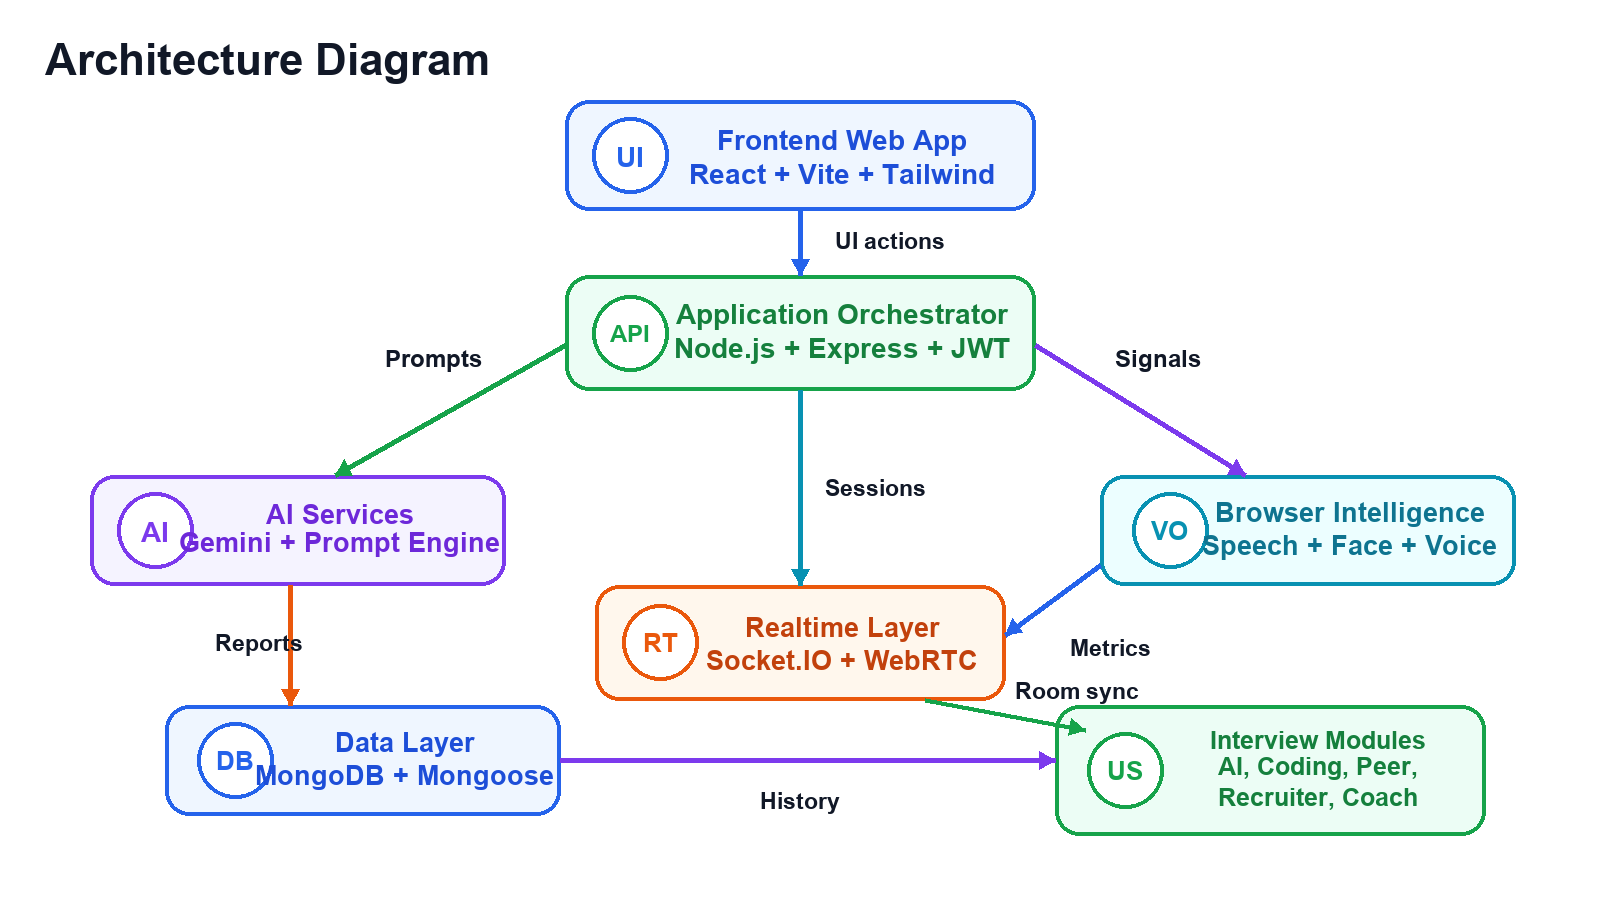
\includegraphics[width=0.95\textwidth]{AI_Driven_Interview_Simulation_Final_Report_assets/figure_02.png}
\caption{Colorful high-level architecture of the AI-driven interview simulation system}
\end{figure}


\section{Development Methodology}

Development Methodology is a central part of the proposed AI-driven interview simulation system because it connects the user-facing experience with measurable recruitment outcomes. In this project, the feature is implemented as part of a browser-based platform where candidates can prepare, recruiters can evaluate, and peers can collaborate without switching between separate tools.


The implementation uses React, Vite, and Tailwind CSS on the client side to keep the user interface responsive and consistent. The backend uses Node.js and Express to expose secure REST APIs, while MongoDB stores users, interview sessions, responses, reports, roadmaps, rooms, and activity history. This separation keeps presentation logic, business logic, and data persistence understandable for maintenance and review.


In the context of iterative full-stack development, the system captures structured inputs from the user and converts them into useful interview actions. These actions include authentication, interview configuration, camera and microphone activation, AI question delivery, answer submission, code execution, peer connection, recruiter scoring, and report generation depending on the selected module.


The major modules involved are requirements analysis, UI design, backend APIs, real-time features, testing, deployment preparation. Their interaction is designed to reduce manual effort while preserving the natural flow of an interview. AI services assist with question generation and coaching, but the application still keeps final data storage, permissions, and workflow control inside the backend server.


The design also considers practical constraints such as browser permissions, network reliability, free deployment limitations, and API quota limits. Therefore, fallback behavior, clear error messages, and modular routing are important engineering decisions in the project. These decisions make the platform suitable for academic demonstration as well as a foundation for future production improvements.


From a software engineering point of view, development methodology is not treated as an isolated screen. It is connected to routing, protected access, backend validation, database persistence, and user feedback. This approach prevents a common problem in student projects where screens look complete but do not share consistent state or saved records.


The project follows a practical full-stack pattern in which the client sends only the required data to the server and the server performs sensitive operations such as authentication, AI API calls, and database writes. This keeps credentials and API keys away from the browser and provides one controlled place to apply error handling, logging, and validation.


For review and testing, this part of the system can be demonstrated through a clear sequence of actions: open the module, submit valid input, observe the server response, inspect stored history, and verify the final user-facing output. This sequence makes the implementation easier to explain during viva and final evaluation because each visible screen maps to a backend responsibility.


The design also improves future maintainability. Since routes, models, and pages are organized by feature, new capabilities such as advanced analytics, stronger coding judge support, multi-provider AI, institution dashboards, or recruiter comparison reports can be added without rewriting the whole application.


\section{Workflow}

Workflow is a central part of the proposed AI-driven interview simulation system because it connects the user-facing experience with measurable recruitment outcomes. In this project, the feature is implemented as part of a browser-based platform where candidates can prepare, recruiters can evaluate, and peers can collaborate without switching between separate tools.


The implementation uses React, Vite, and Tailwind CSS on the client side to keep the user interface responsive and consistent. The backend uses Node.js and Express to expose secure REST APIs, while MongoDB stores users, interview sessions, responses, reports, roadmaps, rooms, and activity history. This separation keeps presentation logic, business logic, and data persistence understandable for maintenance and review.


In the context of candidate and recruiter workflows, the system captures structured inputs from the user and converts them into useful interview actions. These actions include authentication, interview configuration, camera and microphone activation, AI question delivery, answer submission, code execution, peer connection, recruiter scoring, and report generation depending on the selected module.


The major modules involved are login, setup, camera activation, AI question flow, response evaluation, report display. Their interaction is designed to reduce manual effort while preserving the natural flow of an interview. AI services assist with question generation and coaching, but the application still keeps final data storage, permissions, and workflow control inside the backend server.


The design also considers practical constraints such as browser permissions, network reliability, free deployment limitations, and API quota limits. Therefore, fallback behavior, clear error messages, and modular routing are important engineering decisions in the project. These decisions make the platform suitable for academic demonstration as well as a foundation for future production improvements.


From a software engineering point of view, workflow is not treated as an isolated screen. It is connected to routing, protected access, backend validation, database persistence, and user feedback. This approach prevents a common problem in student projects where screens look complete but do not share consistent state or saved records.


The project follows a practical full-stack pattern in which the client sends only the required data to the server and the server performs sensitive operations such as authentication, AI API calls, and database writes. This keeps credentials and API keys away from the browser and provides one controlled place to apply error handling, logging, and validation.


For review and testing, this part of the system can be demonstrated through a clear sequence of actions: open the module, submit valid input, observe the server response, inspect stored history, and verify the final user-facing output. This sequence makes the implementation easier to explain during viva and final evaluation because each visible screen maps to a backend responsibility.


The design also improves future maintainability. Since routes, models, and pages are organized by feature, new capabilities such as advanced analytics, stronger coding judge support, multi-provider AI, institution dashboards, or recruiter comparison reports can be added without rewriting the whole application.


\begin{figure}[H]
\centering
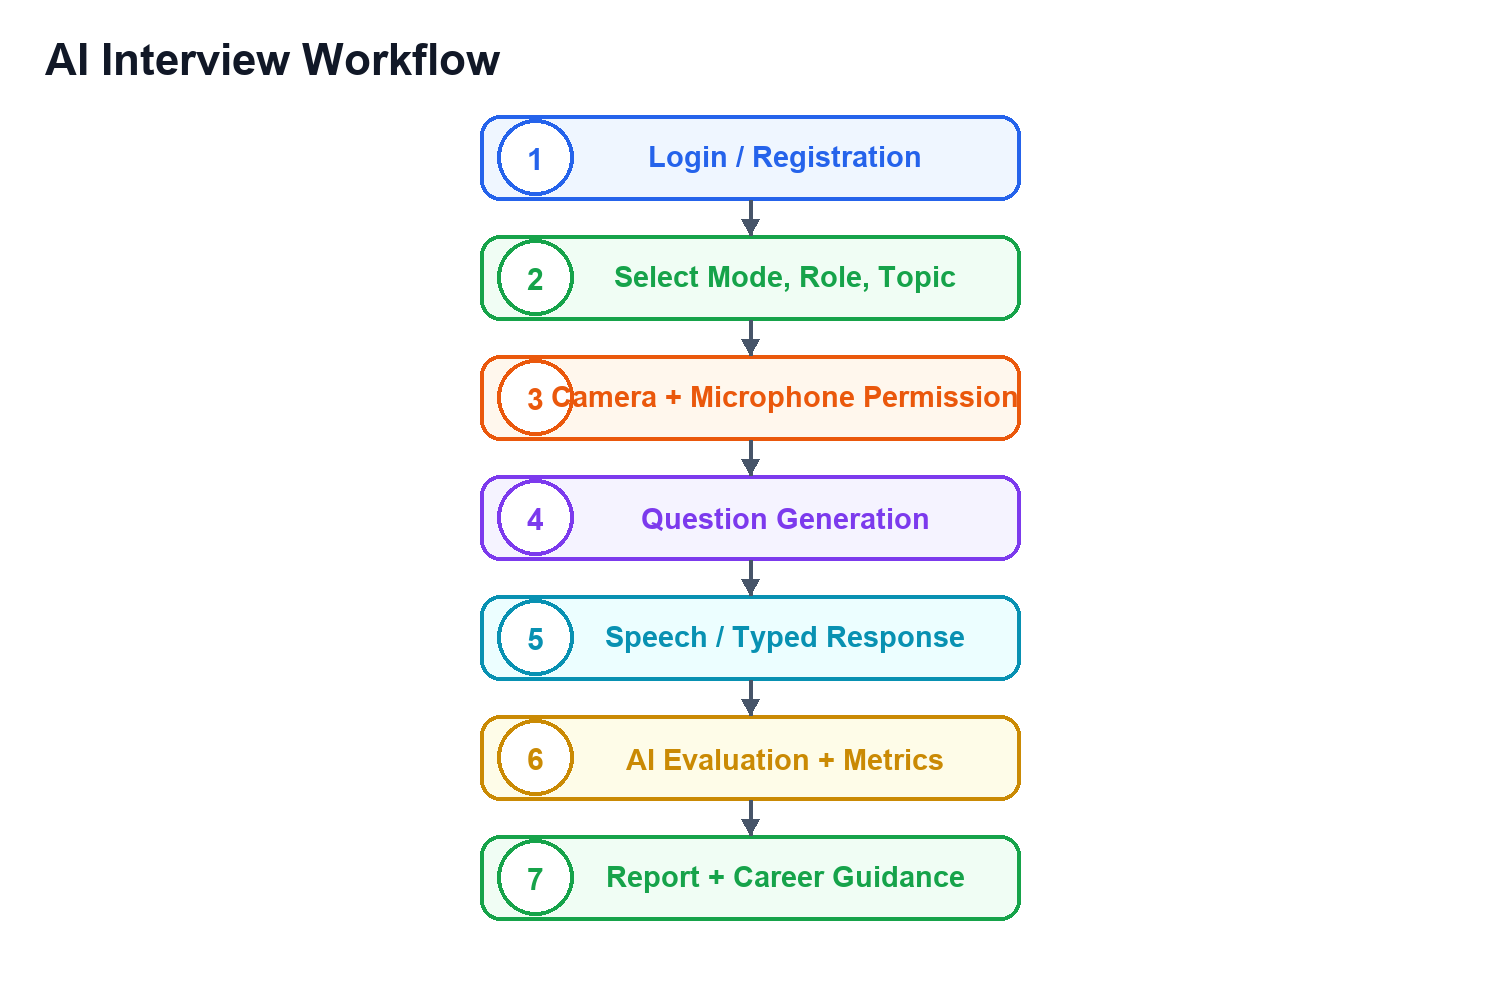
\includegraphics[width=0.95\textwidth]{AI_Driven_Interview_Simulation_Final_Report_assets/figure_03.png}
\caption{AI interview workflow from authentication to final report}
\end{figure}


\section{Flowchart}

Flowchart is a central part of the proposed AI-driven interview simulation system because it connects the user-facing experience with measurable recruitment outcomes. In this project, the feature is implemented as part of a browser-based platform where candidates can prepare, recruiters can evaluate, and peers can collaborate without switching between separate tools.


The implementation uses React, Vite, and Tailwind CSS on the client side to keep the user interface responsive and consistent. The backend uses Node.js and Express to expose secure REST APIs, while MongoDB stores users, interview sessions, responses, reports, roadmaps, rooms, and activity history. This separation keeps presentation logic, business logic, and data persistence understandable for maintenance and review.


In the context of system execution flow, the system captures structured inputs from the user and converts them into useful interview actions. These actions include authentication, interview configuration, camera and microphone activation, AI question delivery, answer submission, code execution, peer connection, recruiter scoring, and report generation depending on the selected module.


The major modules involved are REST APIs, Socket.IO rooms, WebRTC streams, database writes, result rendering. Their interaction is designed to reduce manual effort while preserving the natural flow of an interview. AI services assist with question generation and coaching, but the application still keeps final data storage, permissions, and workflow control inside the backend server.


The design also considers practical constraints such as browser permissions, network reliability, free deployment limitations, and API quota limits. Therefore, fallback behavior, clear error messages, and modular routing are important engineering decisions in the project. These decisions make the platform suitable for academic demonstration as well as a foundation for future production improvements.


From a software engineering point of view, flowchart is not treated as an isolated screen. It is connected to routing, protected access, backend validation, database persistence, and user feedback. This approach prevents a common problem in student projects where screens look complete but do not share consistent state or saved records.


The project follows a practical full-stack pattern in which the client sends only the required data to the server and the server performs sensitive operations such as authentication, AI API calls, and database writes. This keeps credentials and API keys away from the browser and provides one controlled place to apply error handling, logging, and validation.


For review and testing, this part of the system can be demonstrated through a clear sequence of actions: open the module, submit valid input, observe the server response, inspect stored history, and verify the final user-facing output. This sequence makes the implementation easier to explain during viva and final evaluation because each visible screen maps to a backend responsibility.


The design also improves future maintainability. Since routes, models, and pages are organized by feature, new capabilities such as advanced analytics, stronger coding judge support, multi-provider AI, institution dashboards, or recruiter comparison reports can be added without rewriting the whole application.


\begin{figure}[H]
\centering
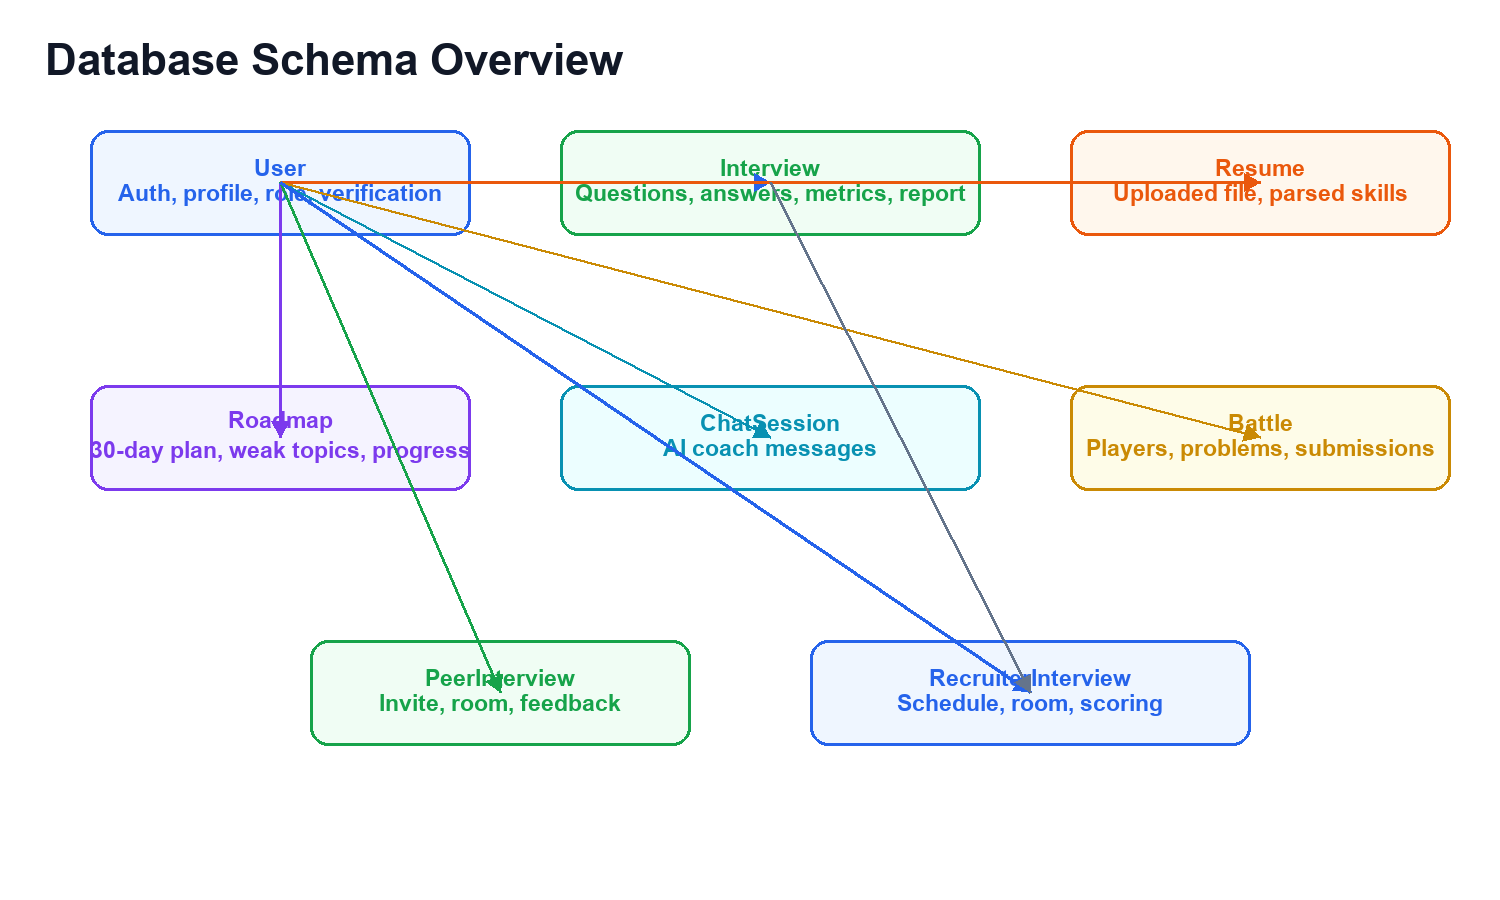
\includegraphics[width=0.95\textwidth]{AI_Driven_Interview_Simulation_Final_Report_assets/figure_04.png}
\caption{Database schema overview and major collection relationships}
\end{figure}


\chapter{IMPLEMENTATION}

\section{User Authentication}

User Authentication is a central part of the proposed AI-driven interview simulation system because it connects the user-facing experience with measurable recruitment outcomes. In this project, the feature is implemented as part of a browser-based platform where candidates can prepare, recruiters can evaluate, and peers can collaborate without switching between separate tools.


The implementation uses React, Vite, and Tailwind CSS on the client side to keep the user interface responsive and consistent. The backend uses Node.js and Express to expose secure REST APIs, while MongoDB stores users, interview sessions, responses, reports, roadmaps, rooms, and activity history. This separation keeps presentation logic, business logic, and data persistence understandable for maintenance and review.


In the context of secure account workflow, the system captures structured inputs from the user and converts them into useful interview actions. These actions include authentication, interview configuration, camera and microphone activation, AI question delivery, answer submission, code execution, peer connection, recruiter scoring, and report generation depending on the selected module.


The major modules involved are registration, email verification, OTP verification, login, reset password, Google sign-in endpoint. Their interaction is designed to reduce manual effort while preserving the natural flow of an interview. AI services assist with question generation and coaching, but the application still keeps final data storage, permissions, and workflow control inside the backend server.


The design also considers practical constraints such as browser permissions, network reliability, free deployment limitations, and API quota limits. Therefore, fallback behavior, clear error messages, and modular routing are important engineering decisions in the project. These decisions make the platform suitable for academic demonstration as well as a foundation for future production improvements.


From a software engineering point of view, user authentication is not treated as an isolated screen. It is connected to routing, protected access, backend validation, database persistence, and user feedback. This approach prevents a common problem in student projects where screens look complete but do not share consistent state or saved records.


The project follows a practical full-stack pattern in which the client sends only the required data to the server and the server performs sensitive operations such as authentication, AI API calls, and database writes. This keeps credentials and API keys away from the browser and provides one controlled place to apply error handling, logging, and validation.


For review and testing, this part of the system can be demonstrated through a clear sequence of actions: open the module, submit valid input, observe the server response, inspect stored history, and verify the final user-facing output. This sequence makes the implementation easier to explain during viva and final evaluation because each visible screen maps to a backend responsibility.


The design also improves future maintainability. Since routes, models, and pages are organized by feature, new capabilities such as advanced analytics, stronger coding judge support, multi-provider AI, institution dashboards, or recruiter comparison reports can be added without rewriting the whole application.


\section{AI Mock Interview Module}

AI Mock Interview Module is a central part of the proposed AI-driven interview simulation system because it connects the user-facing experience with measurable recruitment outcomes. In this project, the feature is implemented as part of a browser-based platform where candidates can prepare, recruiters can evaluate, and peers can collaborate without switching between separate tools.


The implementation uses React, Vite, and Tailwind CSS on the client side to keep the user interface responsive and consistent. The backend uses Node.js and Express to expose secure REST APIs, while MongoDB stores users, interview sessions, responses, reports, roadmaps, rooms, and activity history. This separation keeps presentation logic, business logic, and data persistence understandable for maintenance and review.


In the context of automated interview simulation, the system captures structured inputs from the user and converts them into useful interview actions. These actions include authentication, interview configuration, camera and microphone activation, AI question delivery, answer submission, code execution, peer connection, recruiter scoring, and report generation depending on the selected module.


The major modules involved are setup page, live interview page, AI question generation, speech input, reports. Their interaction is designed to reduce manual effort while preserving the natural flow of an interview. AI services assist with question generation and coaching, but the application still keeps final data storage, permissions, and workflow control inside the backend server.


The design also considers practical constraints such as browser permissions, network reliability, free deployment limitations, and API quota limits. Therefore, fallback behavior, clear error messages, and modular routing are important engineering decisions in the project. These decisions make the platform suitable for academic demonstration as well as a foundation for future production improvements.


From a software engineering point of view, ai mock interview module is not treated as an isolated screen. It is connected to routing, protected access, backend validation, database persistence, and user feedback. This approach prevents a common problem in student projects where screens look complete but do not share consistent state or saved records.


The project follows a practical full-stack pattern in which the client sends only the required data to the server and the server performs sensitive operations such as authentication, AI API calls, and database writes. This keeps credentials and API keys away from the browser and provides one controlled place to apply error handling, logging, and validation.


For review and testing, this part of the system can be demonstrated through a clear sequence of actions: open the module, submit valid input, observe the server response, inspect stored history, and verify the final user-facing output. This sequence makes the implementation easier to explain during viva and final evaluation because each visible screen maps to a backend responsibility.


The design also improves future maintainability. Since routes, models, and pages are organized by feature, new capabilities such as advanced analytics, stronger coding judge support, multi-provider AI, institution dashboards, or recruiter comparison reports can be added without rewriting the whole application.


\section{Competitive Coding Battle}

Competitive Coding Battle is a central part of the proposed AI-driven interview simulation system because it connects the user-facing experience with measurable recruitment outcomes. In this project, the feature is implemented as part of a browser-based platform where candidates can prepare, recruiters can evaluate, and peers can collaborate without switching between separate tools.


The implementation uses React, Vite, and Tailwind CSS on the client side to keep the user interface responsive and consistent. The backend uses Node.js and Express to expose secure REST APIs, while MongoDB stores users, interview sessions, responses, reports, roadmaps, rooms, and activity history. This separation keeps presentation logic, business logic, and data persistence understandable for maintenance and review.


In the context of competitive programming practice, the system captures structured inputs from the user and converts them into useful interview actions. These actions include authentication, interview configuration, camera and microphone activation, AI question delivery, answer submission, code execution, peer connection, recruiter scoring, and report generation depending on the selected module.


The major modules involved are battle lobby, battle arena, Socket.IO synchronization, code submission. Their interaction is designed to reduce manual effort while preserving the natural flow of an interview. AI services assist with question generation and coaching, but the application still keeps final data storage, permissions, and workflow control inside the backend server.


The design also considers practical constraints such as browser permissions, network reliability, free deployment limitations, and API quota limits. Therefore, fallback behavior, clear error messages, and modular routing are important engineering decisions in the project. These decisions make the platform suitable for academic demonstration as well as a foundation for future production improvements.


From a software engineering point of view, competitive coding battle is not treated as an isolated screen. It is connected to routing, protected access, backend validation, database persistence, and user feedback. This approach prevents a common problem in student projects where screens look complete but do not share consistent state or saved records.


The project follows a practical full-stack pattern in which the client sends only the required data to the server and the server performs sensitive operations such as authentication, AI API calls, and database writes. This keeps credentials and API keys away from the browser and provides one controlled place to apply error handling, logging, and validation.


For review and testing, this part of the system can be demonstrated through a clear sequence of actions: open the module, submit valid input, observe the server response, inspect stored history, and verify the final user-facing output. This sequence makes the implementation easier to explain during viva and final evaluation because each visible screen maps to a backend responsibility.


The design also improves future maintainability. Since routes, models, and pages are organized by feature, new capabilities such as advanced analytics, stronger coding judge support, multi-provider AI, institution dashboards, or recruiter comparison reports can be added without rewriting the whole application.


\section{Peer Mock Interview}

Peer Mock Interview is a central part of the proposed AI-driven interview simulation system because it connects the user-facing experience with measurable recruitment outcomes. In this project, the feature is implemented as part of a browser-based platform where candidates can prepare, recruiters can evaluate, and peers can collaborate without switching between separate tools.


The implementation uses React, Vite, and Tailwind CSS on the client side to keep the user interface responsive and consistent. The backend uses Node.js and Express to expose secure REST APIs, while MongoDB stores users, interview sessions, responses, reports, roadmaps, rooms, and activity history. This separation keeps presentation logic, business logic, and data persistence understandable for maintenance and review.


In the context of collaborative interview practice, the system captures structured inputs from the user and converts them into useful interview actions. These actions include authentication, interview configuration, camera and microphone activation, AI question delivery, answer submission, code execution, peer connection, recruiter scoring, and report generation depending on the selected module.


The major modules involved are candidate discovery, invitations, peer rooms, feedback history. Their interaction is designed to reduce manual effort while preserving the natural flow of an interview. AI services assist with question generation and coaching, but the application still keeps final data storage, permissions, and workflow control inside the backend server.


The design also considers practical constraints such as browser permissions, network reliability, free deployment limitations, and API quota limits. Therefore, fallback behavior, clear error messages, and modular routing are important engineering decisions in the project. These decisions make the platform suitable for academic demonstration as well as a foundation for future production improvements.


From a software engineering point of view, peer mock interview is not treated as an isolated screen. It is connected to routing, protected access, backend validation, database persistence, and user feedback. This approach prevents a common problem in student projects where screens look complete but do not share consistent state or saved records.


The project follows a practical full-stack pattern in which the client sends only the required data to the server and the server performs sensitive operations such as authentication, AI API calls, and database writes. This keeps credentials and API keys away from the browser and provides one controlled place to apply error handling, logging, and validation.


For review and testing, this part of the system can be demonstrated through a clear sequence of actions: open the module, submit valid input, observe the server response, inspect stored history, and verify the final user-facing output. This sequence makes the implementation easier to explain during viva and final evaluation because each visible screen maps to a backend responsibility.


The design also improves future maintainability. Since routes, models, and pages are organized by feature, new capabilities such as advanced analytics, stronger coding judge support, multi-provider AI, institution dashboards, or recruiter comparison reports can be added without rewriting the whole application.


\section{Recruiter Live Interview Portal}

Recruiter Live Interview Portal is a central part of the proposed AI-driven interview simulation system because it connects the user-facing experience with measurable recruitment outcomes. In this project, the feature is implemented as part of a browser-based platform where candidates can prepare, recruiters can evaluate, and peers can collaborate without switching between separate tools.


The implementation uses React, Vite, and Tailwind CSS on the client side to keep the user interface responsive and consistent. The backend uses Node.js and Express to expose secure REST APIs, while MongoDB stores users, interview sessions, responses, reports, roadmaps, rooms, and activity history. This separation keeps presentation logic, business logic, and data persistence understandable for maintenance and review.


In the context of professional hiring workflow, the system captures structured inputs from the user and converts them into useful interview actions. These actions include authentication, interview configuration, camera and microphone activation, AI question delivery, answer submission, code execution, peer connection, recruiter scoring, and report generation depending on the selected module.


The major modules involved are schedule creation, recruiter dashboard, live room, scoring, recording metadata. Their interaction is designed to reduce manual effort while preserving the natural flow of an interview. AI services assist with question generation and coaching, but the application still keeps final data storage, permissions, and workflow control inside the backend server.


The design also considers practical constraints such as browser permissions, network reliability, free deployment limitations, and API quota limits. Therefore, fallback behavior, clear error messages, and modular routing are important engineering decisions in the project. These decisions make the platform suitable for academic demonstration as well as a foundation for future production improvements.


From a software engineering point of view, recruiter live interview portal is not treated as an isolated screen. It is connected to routing, protected access, backend validation, database persistence, and user feedback. This approach prevents a common problem in student projects where screens look complete but do not share consistent state or saved records.


The project follows a practical full-stack pattern in which the client sends only the required data to the server and the server performs sensitive operations such as authentication, AI API calls, and database writes. This keeps credentials and API keys away from the browser and provides one controlled place to apply error handling, logging, and validation.


For review and testing, this part of the system can be demonstrated through a clear sequence of actions: open the module, submit valid input, observe the server response, inspect stored history, and verify the final user-facing output. This sequence makes the implementation easier to explain during viva and final evaluation because each visible screen maps to a backend responsibility.


The design also improves future maintainability. Since routes, models, and pages are organized by feature, new capabilities such as advanced analytics, stronger coding judge support, multi-provider AI, institution dashboards, or recruiter comparison reports can be added without rewriting the whole application.


\section{Career Roadmap \& AI Coach}

Career Roadmap \& AI Coach is a central part of the proposed AI-driven interview simulation system because it connects the user-facing experience with measurable recruitment outcomes. In this project, the feature is implemented as part of a browser-based platform where candidates can prepare, recruiters can evaluate, and peers can collaborate without switching between separate tools.


The implementation uses React, Vite, and Tailwind CSS on the client side to keep the user interface responsive and consistent. The backend uses Node.js and Express to expose secure REST APIs, while MongoDB stores users, interview sessions, responses, reports, roadmaps, rooms, and activity history. This separation keeps presentation logic, business logic, and data persistence understandable for maintenance and review.


In the context of continuous preparation support, the system captures structured inputs from the user and converts them into useful interview actions. These actions include authentication, interview configuration, camera and microphone activation, AI question delivery, answer submission, code execution, peer connection, recruiter scoring, and report generation depending on the selected module.


The major modules involved are roadmap generation, roadmap progress, coach sessions, chat messages. Their interaction is designed to reduce manual effort while preserving the natural flow of an interview. AI services assist with question generation and coaching, but the application still keeps final data storage, permissions, and workflow control inside the backend server.


The design also considers practical constraints such as browser permissions, network reliability, free deployment limitations, and API quota limits. Therefore, fallback behavior, clear error messages, and modular routing are important engineering decisions in the project. These decisions make the platform suitable for academic demonstration as well as a foundation for future production improvements.


From a software engineering point of view, career roadmap \& ai coach is not treated as an isolated screen. It is connected to routing, protected access, backend validation, database persistence, and user feedback. This approach prevents a common problem in student projects where screens look complete but do not share consistent state or saved records.


The project follows a practical full-stack pattern in which the client sends only the required data to the server and the server performs sensitive operations such as authentication, AI API calls, and database writes. This keeps credentials and API keys away from the browser and provides one controlled place to apply error handling, logging, and validation.


For review and testing, this part of the system can be demonstrated through a clear sequence of actions: open the module, submit valid input, observe the server response, inspect stored history, and verify the final user-facing output. This sequence makes the implementation easier to explain during viva and final evaluation because each visible screen maps to a backend responsibility.


The design also improves future maintainability. Since routes, models, and pages are organized by feature, new capabilities such as advanced analytics, stronger coding judge support, multi-provider AI, institution dashboards, or recruiter comparison reports can be added without rewriting the whole application.


\section{Database Design}

Database Design is a central part of the proposed AI-driven interview simulation system because it connects the user-facing experience with measurable recruitment outcomes. In this project, the feature is implemented as part of a browser-based platform where candidates can prepare, recruiters can evaluate, and peers can collaborate without switching between separate tools.


The implementation uses React, Vite, and Tailwind CSS on the client side to keep the user interface responsive and consistent. The backend uses Node.js and Express to expose secure REST APIs, while MongoDB stores users, interview sessions, responses, reports, roadmaps, rooms, and activity history. This separation keeps presentation logic, business logic, and data persistence understandable for maintenance and review.


In the context of persistent storage, the system captures structured inputs from the user and converts them into useful interview actions. These actions include authentication, interview configuration, camera and microphone activation, AI question delivery, answer submission, code execution, peer connection, recruiter scoring, and report generation depending on the selected module.


The major modules involved are User, Interview, Resume, Roadmap, ChatSession, Battle, PeerInterview, RecruiterInterview models. Their interaction is designed to reduce manual effort while preserving the natural flow of an interview. AI services assist with question generation and coaching, but the application still keeps final data storage, permissions, and workflow control inside the backend server.


The design also considers practical constraints such as browser permissions, network reliability, free deployment limitations, and API quota limits. Therefore, fallback behavior, clear error messages, and modular routing are important engineering decisions in the project. These decisions make the platform suitable for academic demonstration as well as a foundation for future production improvements.


From a software engineering point of view, database design is not treated as an isolated screen. It is connected to routing, protected access, backend validation, database persistence, and user feedback. This approach prevents a common problem in student projects where screens look complete but do not share consistent state or saved records.


The project follows a practical full-stack pattern in which the client sends only the required data to the server and the server performs sensitive operations such as authentication, AI API calls, and database writes. This keeps credentials and API keys away from the browser and provides one controlled place to apply error handling, logging, and validation.


For review and testing, this part of the system can be demonstrated through a clear sequence of actions: open the module, submit valid input, observe the server response, inspect stored history, and verify the final user-facing output. This sequence makes the implementation easier to explain during viva and final evaluation because each visible screen maps to a backend responsibility.


The design also improves future maintainability. Since routes, models, and pages are organized by feature, new capabilities such as advanced analytics, stronger coding judge support, multi-provider AI, institution dashboards, or recruiter comparison reports can be added without rewriting the whole application.


\begin{longtable}{|>{\raggedright\arraybackslash}p{0.31\textwidth}|>{\raggedright\arraybackslash}p{0.31\textwidth}|>{\raggedright\arraybackslash}p{0.31\textwidth}|}
\hline
Collection & Main Data Stored & Used By \\
\hline
\endfirsthead
\hline
Collection & Main Data Stored & Used By \\
\hline
\endhead
users & Name, email, password hash, roles, verification state & Authentication and authorization \\
\hline
interviews & Setup, questions, answers, metrics, report & AI interview and reports \\
\hline
resumes & Uploaded document metadata and parsed text & Resume-based personalization \\
\hline
roadmaps & Generated learning plan, weak topics, progress & Career roadmap \\
\hline
chatSessions & Coach conversation and messages & AI coach \\
\hline
battles & Players, problems, submissions, result & Coding battle \\
\hline
peerInterviews & Peer room, participants, feedback & Peer mock interview \\
\hline
recruiterInterviews & Schedule, recruiter room, candidate score & Recruiter portal \\
\hline
\end{longtable}

\section{API Integration}

API Integration is a central part of the proposed AI-driven interview simulation system because it connects the user-facing experience with measurable recruitment outcomes. In this project, the feature is implemented as part of a browser-based platform where candidates can prepare, recruiters can evaluate, and peers can collaborate without switching between separate tools.


The implementation uses React, Vite, and Tailwind CSS on the client side to keep the user interface responsive and consistent. The backend uses Node.js and Express to expose secure REST APIs, while MongoDB stores users, interview sessions, responses, reports, roadmaps, rooms, and activity history. This separation keeps presentation logic, business logic, and data persistence understandable for maintenance and review.


In the context of frontend-backend connectivity, the system captures structured inputs from the user and converts them into useful interview actions. These actions include authentication, interview configuration, camera and microphone activation, AI question delivery, answer submission, code execution, peer connection, recruiter scoring, and report generation depending on the selected module.


The major modules involved are auth routes, interview routes, code routes, peer routes, recruiter routes, roadmap routes. Their interaction is designed to reduce manual effort while preserving the natural flow of an interview. AI services assist with question generation and coaching, but the application still keeps final data storage, permissions, and workflow control inside the backend server.


The design also considers practical constraints such as browser permissions, network reliability, free deployment limitations, and API quota limits. Therefore, fallback behavior, clear error messages, and modular routing are important engineering decisions in the project. These decisions make the platform suitable for academic demonstration as well as a foundation for future production improvements.


From a software engineering point of view, api integration is not treated as an isolated screen. It is connected to routing, protected access, backend validation, database persistence, and user feedback. This approach prevents a common problem in student projects where screens look complete but do not share consistent state or saved records.


The project follows a practical full-stack pattern in which the client sends only the required data to the server and the server performs sensitive operations such as authentication, AI API calls, and database writes. This keeps credentials and API keys away from the browser and provides one controlled place to apply error handling, logging, and validation.


For review and testing, this part of the system can be demonstrated through a clear sequence of actions: open the module, submit valid input, observe the server response, inspect stored history, and verify the final user-facing output. This sequence makes the implementation easier to explain during viva and final evaluation because each visible screen maps to a backend responsibility.


The design also improves future maintainability. Since routes, models, and pages are organized by feature, new capabilities such as advanced analytics, stronger coding judge support, multi-provider AI, institution dashboards, or recruiter comparison reports can be added without rewriting the whole application.


\begin{longtable}{|>{\raggedright\arraybackslash}p{0.31\textwidth}|>{\raggedright\arraybackslash}p{0.31\textwidth}|>{\raggedright\arraybackslash}p{0.31\textwidth}|}
\hline
API Group & Base Route & Important Endpoints \\
\hline
\endfirsthead
\hline
API Group & Base Route & Important Endpoints \\
\hline
\endhead
Authentication & /api/auth & register, login, google, verify-otp, resend-otp, forgot-password, reset-password, me \\
\hline
Interviews & /api/interviews & setup, history/me, answer, skip, complete, report, proctoring-violation \\
\hline
Code Runner & /api/code & run, submit \\
\hline
Roadmaps & /api/roadmaps & generate, list, detail, complete day, delete \\
\hline
Coach & /api/coach & sessions, messages, update, delete \\
\hline
Peer & /api/peer & candidates, invite, invitations, room, feedback, history \\
\hline
Recruiter & /api/recruiter & schedule, interviews, room, score, recording \\
\hline
Resume & /api/resumes & upload, parse, list, delete \\
\hline
Admin & /api/admin & admin dashboard and management operations \\
\hline
\end{longtable}

\chapter{RESULTS AND ANALYSIS}

\section{Functional Testing}

Functional Testing is a central part of the proposed AI-driven interview simulation system because it connects the user-facing experience with measurable recruitment outcomes. In this project, the feature is implemented as part of a browser-based platform where candidates can prepare, recruiters can evaluate, and peers can collaborate without switching between separate tools.


The implementation uses React, Vite, and Tailwind CSS on the client side to keep the user interface responsive and consistent. The backend uses Node.js and Express to expose secure REST APIs, while MongoDB stores users, interview sessions, responses, reports, roadmaps, rooms, and activity history. This separation keeps presentation logic, business logic, and data persistence understandable for maintenance and review.


In the context of feature verification, the system captures structured inputs from the user and converts them into useful interview actions. These actions include authentication, interview configuration, camera and microphone activation, AI question delivery, answer submission, code execution, peer connection, recruiter scoring, and report generation depending on the selected module.


The major modules involved are auth, AI interview, coding, battle, peer, recruiter, roadmap, coach. Their interaction is designed to reduce manual effort while preserving the natural flow of an interview. AI services assist with question generation and coaching, but the application still keeps final data storage, permissions, and workflow control inside the backend server.


The design also considers practical constraints such as browser permissions, network reliability, free deployment limitations, and API quota limits. Therefore, fallback behavior, clear error messages, and modular routing are important engineering decisions in the project. These decisions make the platform suitable for academic demonstration as well as a foundation for future production improvements.


From a software engineering point of view, functional testing is not treated as an isolated screen. It is connected to routing, protected access, backend validation, database persistence, and user feedback. This approach prevents a common problem in student projects where screens look complete but do not share consistent state or saved records.


The project follows a practical full-stack pattern in which the client sends only the required data to the server and the server performs sensitive operations such as authentication, AI API calls, and database writes. This keeps credentials and API keys away from the browser and provides one controlled place to apply error handling, logging, and validation.


For review and testing, this part of the system can be demonstrated through a clear sequence of actions: open the module, submit valid input, observe the server response, inspect stored history, and verify the final user-facing output. This sequence makes the implementation easier to explain during viva and final evaluation because each visible screen maps to a backend responsibility.


The design also improves future maintainability. Since routes, models, and pages are organized by feature, new capabilities such as advanced analytics, stronger coding judge support, multi-provider AI, institution dashboards, or recruiter comparison reports can be added without rewriting the whole application.


\begin{longtable}{|>{\raggedright\arraybackslash}p{0.19\textwidth}|>{\raggedright\arraybackslash}p{0.19\textwidth}|>{\raggedright\arraybackslash}p{0.19\textwidth}|>{\raggedright\arraybackslash}p{0.19\textwidth}|>{\raggedright\arraybackslash}p{0.19\textwidth}|}
\hline
Test ID & Module & Scenario & Expected Result & Status \\
\hline
\endfirsthead
\hline
Test ID & Module & Scenario & Expected Result & Status \\
\hline
\endhead
TC-01 & Authentication & Register with valid email and password & OTP sent and verification screen shown & Pass \\
\hline
TC-02 & Authentication & Login before verification & Meaningful verification error shown & Pass \\
\hline
TC-03 & AI Interview & Start role-based interview & First question displayed and answer accepted & Pass \\
\hline
TC-04 & Coding Interview & Run sample solution & Visible test result section updates & Pass \\
\hline
TC-05 & Coding Battle & Join battle lobby & Battle room opens with problem and editor & Pass \\
\hline
TC-06 & Peer Interview & Send peer request & Invitation appears for receiver & Pass \\
\hline
TC-07 & Recruiter Portal & Schedule interview & Room and candidate details are stored & Pass \\
\hline
TC-08 & Roadmap & Generate roadmap by weak topic & Roadmap card and daily plan are created & Pass \\
\hline
\end{longtable}

\section{Performance Analysis}

Performance Analysis is a central part of the proposed AI-driven interview simulation system because it connects the user-facing experience with measurable recruitment outcomes. In this project, the feature is implemented as part of a browser-based platform where candidates can prepare, recruiters can evaluate, and peers can collaborate without switching between separate tools.


The implementation uses React, Vite, and Tailwind CSS on the client side to keep the user interface responsive and consistent. The backend uses Node.js and Express to expose secure REST APIs, while MongoDB stores users, interview sessions, responses, reports, roadmaps, rooms, and activity history. This separation keeps presentation logic, business logic, and data persistence understandable for maintenance and review.


In the context of runtime observations, the system captures structured inputs from the user and converts them into useful interview actions. These actions include authentication, interview configuration, camera and microphone activation, AI question delivery, answer submission, code execution, peer connection, recruiter scoring, and report generation depending on the selected module.


The major modules involved are page load, API calls, database persistence, real-time communication. Their interaction is designed to reduce manual effort while preserving the natural flow of an interview. AI services assist with question generation and coaching, but the application still keeps final data storage, permissions, and workflow control inside the backend server.


The design also considers practical constraints such as browser permissions, network reliability, free deployment limitations, and API quota limits. Therefore, fallback behavior, clear error messages, and modular routing are important engineering decisions in the project. These decisions make the platform suitable for academic demonstration as well as a foundation for future production improvements.


From a software engineering point of view, performance analysis is not treated as an isolated screen. It is connected to routing, protected access, backend validation, database persistence, and user feedback. This approach prevents a common problem in student projects where screens look complete but do not share consistent state or saved records.


The project follows a practical full-stack pattern in which the client sends only the required data to the server and the server performs sensitive operations such as authentication, AI API calls, and database writes. This keeps credentials and API keys away from the browser and provides one controlled place to apply error handling, logging, and validation.


For review and testing, this part of the system can be demonstrated through a clear sequence of actions: open the module, submit valid input, observe the server response, inspect stored history, and verify the final user-facing output. This sequence makes the implementation easier to explain during viva and final evaluation because each visible screen maps to a backend responsibility.


The design also improves future maintainability. Since routes, models, and pages are organized by feature, new capabilities such as advanced analytics, stronger coding judge support, multi-provider AI, institution dashboards, or recruiter comparison reports can be added without rewriting the whole application.


\begin{longtable}{|>{\raggedright\arraybackslash}p{0.23\textwidth}|>{\raggedright\arraybackslash}p{0.23\textwidth}|>{\raggedright\arraybackslash}p{0.23\textwidth}|>{\raggedright\arraybackslash}p{0.23\textwidth}|}
\hline
Module & Observed Operation & Performance Consideration & Optimization Used \\
\hline
\endfirsthead
\hline
Module & Observed Operation & Performance Consideration & Optimization Used \\
\hline
\endhead
Frontend & Route navigation and dashboards & Should remain responsive & Vite build and component-based pages \\
\hline
API Server & Authenticated REST requests & Should respond predictably & Express middleware and route separation \\
\hline
Database & Interview and session persistence & Should support nested results & Mongoose schema design \\
\hline
AI Service & Question and roadmap generation & Dependent on quota and response time & Backend-only calls and fallback handling \\
\hline
Realtime & Peer and battle rooms & Requires low latency & Socket.IO and WebRTC support \\
\hline
\end{longtable}

\section{AI Interview Evaluation}

AI Interview Evaluation is a central part of the proposed AI-driven interview simulation system because it connects the user-facing experience with measurable recruitment outcomes. In this project, the feature is implemented as part of a browser-based platform where candidates can prepare, recruiters can evaluate, and peers can collaborate without switching between separate tools.


The implementation uses React, Vite, and Tailwind CSS on the client side to keep the user interface responsive and consistent. The backend uses Node.js and Express to expose secure REST APIs, while MongoDB stores users, interview sessions, responses, reports, roadmaps, rooms, and activity history. This separation keeps presentation logic, business logic, and data persistence understandable for maintenance and review.


In the context of quality of AI-supported feedback, the system captures structured inputs from the user and converts them into useful interview actions. These actions include authentication, interview configuration, camera and microphone activation, AI question delivery, answer submission, code execution, peer connection, recruiter scoring, and report generation depending on the selected module.


The major modules involved are answer content, communication, confidence, report narrative. Their interaction is designed to reduce manual effort while preserving the natural flow of an interview. AI services assist with question generation and coaching, but the application still keeps final data storage, permissions, and workflow control inside the backend server.


The design also considers practical constraints such as browser permissions, network reliability, free deployment limitations, and API quota limits. Therefore, fallback behavior, clear error messages, and modular routing are important engineering decisions in the project. These decisions make the platform suitable for academic demonstration as well as a foundation for future production improvements.


From a software engineering point of view, ai interview evaluation is not treated as an isolated screen. It is connected to routing, protected access, backend validation, database persistence, and user feedback. This approach prevents a common problem in student projects where screens look complete but do not share consistent state or saved records.


The project follows a practical full-stack pattern in which the client sends only the required data to the server and the server performs sensitive operations such as authentication, AI API calls, and database writes. This keeps credentials and API keys away from the browser and provides one controlled place to apply error handling, logging, and validation.


For review and testing, this part of the system can be demonstrated through a clear sequence of actions: open the module, submit valid input, observe the server response, inspect stored history, and verify the final user-facing output. This sequence makes the implementation easier to explain during viva and final evaluation because each visible screen maps to a backend responsibility.


The design also improves future maintainability. Since routes, models, and pages are organized by feature, new capabilities such as advanced analytics, stronger coding judge support, multi-provider AI, institution dashboards, or recruiter comparison reports can be added without rewriting the whole application.


\begin{longtable}{|>{\raggedright\arraybackslash}p{0.31\textwidth}|>{\raggedright\arraybackslash}p{0.31\textwidth}|>{\raggedright\arraybackslash}p{0.31\textwidth}|}
\hline
Metric & Meaning & How It Helps Candidate \\
\hline
\endfirsthead
\hline
Metric & Meaning & How It Helps Candidate \\
\hline
\endhead
Content Score & Measures correctness and completeness of answer & Improves technical preparation \\
\hline
Confidence & Indicates delivery quality and posture signals & Improves communication style \\
\hline
Fluency & Captures response smoothness and hesitation & Reduces interview anxiety \\
\hline
Eye Contact & Estimates focus using browser camera analysis & Encourages professional presence \\
\hline
Recommendation & Summarizes next steps & Provides actionable preparation plan \\
\hline
\end{longtable}

\section{Recruiter Module Results}

Recruiter Module Results is a central part of the proposed AI-driven interview simulation system because it connects the user-facing experience with measurable recruitment outcomes. In this project, the feature is implemented as part of a browser-based platform where candidates can prepare, recruiters can evaluate, and peers can collaborate without switching between separate tools.


The implementation uses React, Vite, and Tailwind CSS on the client side to keep the user interface responsive and consistent. The backend uses Node.js and Express to expose secure REST APIs, while MongoDB stores users, interview sessions, responses, reports, roadmaps, rooms, and activity history. This separation keeps presentation logic, business logic, and data persistence understandable for maintenance and review.


In the context of live recruiter workflow, the system captures structured inputs from the user and converts them into useful interview actions. These actions include authentication, interview configuration, camera and microphone activation, AI question delivery, answer submission, code execution, peer connection, recruiter scoring, and report generation depending on the selected module.


The major modules involved are scheduling, room link, scoring, candidate record. Their interaction is designed to reduce manual effort while preserving the natural flow of an interview. AI services assist with question generation and coaching, but the application still keeps final data storage, permissions, and workflow control inside the backend server.


The design also considers practical constraints such as browser permissions, network reliability, free deployment limitations, and API quota limits. Therefore, fallback behavior, clear error messages, and modular routing are important engineering decisions in the project. These decisions make the platform suitable for academic demonstration as well as a foundation for future production improvements.


From a software engineering point of view, recruiter module results is not treated as an isolated screen. It is connected to routing, protected access, backend validation, database persistence, and user feedback. This approach prevents a common problem in student projects where screens look complete but do not share consistent state or saved records.


The project follows a practical full-stack pattern in which the client sends only the required data to the server and the server performs sensitive operations such as authentication, AI API calls, and database writes. This keeps credentials and API keys away from the browser and provides one controlled place to apply error handling, logging, and validation.


For review and testing, this part of the system can be demonstrated through a clear sequence of actions: open the module, submit valid input, observe the server response, inspect stored history, and verify the final user-facing output. This sequence makes the implementation easier to explain during viva and final evaluation because each visible screen maps to a backend responsibility.


The design also improves future maintainability. Since routes, models, and pages are organized by feature, new capabilities such as advanced analytics, stronger coding judge support, multi-provider AI, institution dashboards, or recruiter comparison reports can be added without rewriting the whole application.


\section{User Feedback}

User Feedback is a central part of the proposed AI-driven interview simulation system because it connects the user-facing experience with measurable recruitment outcomes. In this project, the feature is implemented as part of a browser-based platform where candidates can prepare, recruiters can evaluate, and peers can collaborate without switching between separate tools.


The implementation uses React, Vite, and Tailwind CSS on the client side to keep the user interface responsive and consistent. The backend uses Node.js and Express to expose secure REST APIs, while MongoDB stores users, interview sessions, responses, reports, roadmaps, rooms, and activity history. This separation keeps presentation logic, business logic, and data persistence understandable for maintenance and review.


In the context of candidate usability observations, the system captures structured inputs from the user and converts them into useful interview actions. These actions include authentication, interview configuration, camera and microphone activation, AI question delivery, answer submission, code execution, peer connection, recruiter scoring, and report generation depending on the selected module.


The major modules involved are clear UI, fast navigation, realistic practice, useful reports. Their interaction is designed to reduce manual effort while preserving the natural flow of an interview. AI services assist with question generation and coaching, but the application still keeps final data storage, permissions, and workflow control inside the backend server.


The design also considers practical constraints such as browser permissions, network reliability, free deployment limitations, and API quota limits. Therefore, fallback behavior, clear error messages, and modular routing are important engineering decisions in the project. These decisions make the platform suitable for academic demonstration as well as a foundation for future production improvements.


From a software engineering point of view, user feedback is not treated as an isolated screen. It is connected to routing, protected access, backend validation, database persistence, and user feedback. This approach prevents a common problem in student projects where screens look complete but do not share consistent state or saved records.


The project follows a practical full-stack pattern in which the client sends only the required data to the server and the server performs sensitive operations such as authentication, AI API calls, and database writes. This keeps credentials and API keys away from the browser and provides one controlled place to apply error handling, logging, and validation.


For review and testing, this part of the system can be demonstrated through a clear sequence of actions: open the module, submit valid input, observe the server response, inspect stored history, and verify the final user-facing output. This sequence makes the implementation easier to explain during viva and final evaluation because each visible screen maps to a backend responsibility.


The design also improves future maintainability. Since routes, models, and pages are organized by feature, new capabilities such as advanced analytics, stronger coding judge support, multi-provider AI, institution dashboards, or recruiter comparison reports can be added without rewriting the whole application.


\section{Discussion}

Discussion is a central part of the proposed AI-driven interview simulation system because it connects the user-facing experience with measurable recruitment outcomes. In this project, the feature is implemented as part of a browser-based platform where candidates can prepare, recruiters can evaluate, and peers can collaborate without switching between separate tools.


The implementation uses React, Vite, and Tailwind CSS on the client side to keep the user interface responsive and consistent. The backend uses Node.js and Express to expose secure REST APIs, while MongoDB stores users, interview sessions, responses, reports, roadmaps, rooms, and activity history. This separation keeps presentation logic, business logic, and data persistence understandable for maintenance and review.


In the context of strengths and limitations, the system captures structured inputs from the user and converts them into useful interview actions. These actions include authentication, interview configuration, camera and microphone activation, AI question delivery, answer submission, code execution, peer connection, recruiter scoring, and report generation depending on the selected module.


The major modules involved are AI dependency, quota limits, browser permissions, network reliability. Their interaction is designed to reduce manual effort while preserving the natural flow of an interview. AI services assist with question generation and coaching, but the application still keeps final data storage, permissions, and workflow control inside the backend server.


The design also considers practical constraints such as browser permissions, network reliability, free deployment limitations, and API quota limits. Therefore, fallback behavior, clear error messages, and modular routing are important engineering decisions in the project. These decisions make the platform suitable for academic demonstration as well as a foundation for future production improvements.


From a software engineering point of view, discussion is not treated as an isolated screen. It is connected to routing, protected access, backend validation, database persistence, and user feedback. This approach prevents a common problem in student projects where screens look complete but do not share consistent state or saved records.


The project follows a practical full-stack pattern in which the client sends only the required data to the server and the server performs sensitive operations such as authentication, AI API calls, and database writes. This keeps credentials and API keys away from the browser and provides one controlled place to apply error handling, logging, and validation.


For review and testing, this part of the system can be demonstrated through a clear sequence of actions: open the module, submit valid input, observe the server response, inspect stored history, and verify the final user-facing output. This sequence makes the implementation easier to explain during viva and final evaluation because each visible screen maps to a backend responsibility.


The design also improves future maintainability. Since routes, models, and pages are organized by feature, new capabilities such as advanced analytics, stronger coding judge support, multi-provider AI, institution dashboards, or recruiter comparison reports can be added without rewriting the whole application.


\chapter{CONCLUSION AND FUTURE SCOPE}

\section{Conclusion}

Conclusion is a central part of the proposed AI-driven interview simulation system because it connects the user-facing experience with measurable recruitment outcomes. In this project, the feature is implemented as part of a browser-based platform where candidates can prepare, recruiters can evaluate, and peers can collaborate without switching between separate tools.


The implementation uses React, Vite, and Tailwind CSS on the client side to keep the user interface responsive and consistent. The backend uses Node.js and Express to expose secure REST APIs, while MongoDB stores users, interview sessions, responses, reports, roadmaps, rooms, and activity history. This separation keeps presentation logic, business logic, and data persistence understandable for maintenance and review.


In the context of project outcome, the system captures structured inputs from the user and converts them into useful interview actions. These actions include authentication, interview configuration, camera and microphone activation, AI question delivery, answer submission, code execution, peer connection, recruiter scoring, and report generation depending on the selected module.


The major modules involved are unified interview simulation, recruitment support, coding practice, reports, AI guidance. Their interaction is designed to reduce manual effort while preserving the natural flow of an interview. AI services assist with question generation and coaching, but the application still keeps final data storage, permissions, and workflow control inside the backend server.


The design also considers practical constraints such as browser permissions, network reliability, free deployment limitations, and API quota limits. Therefore, fallback behavior, clear error messages, and modular routing are important engineering decisions in the project. These decisions make the platform suitable for academic demonstration as well as a foundation for future production improvements.


From a software engineering point of view, conclusion is not treated as an isolated screen. It is connected to routing, protected access, backend validation, database persistence, and user feedback. This approach prevents a common problem in student projects where screens look complete but do not share consistent state or saved records.


The project follows a practical full-stack pattern in which the client sends only the required data to the server and the server performs sensitive operations such as authentication, AI API calls, and database writes. This keeps credentials and API keys away from the browser and provides one controlled place to apply error handling, logging, and validation.


For review and testing, this part of the system can be demonstrated through a clear sequence of actions: open the module, submit valid input, observe the server response, inspect stored history, and verify the final user-facing output. This sequence makes the implementation easier to explain during viva and final evaluation because each visible screen maps to a backend responsibility.


The design also improves future maintainability. Since routes, models, and pages are organized by feature, new capabilities such as advanced analytics, stronger coding judge support, multi-provider AI, institution dashboards, or recruiter comparison reports can be added without rewriting the whole application.


\section{Future Scope}

Future Scope is a central part of the proposed AI-driven interview simulation system because it connects the user-facing experience with measurable recruitment outcomes. In this project, the feature is implemented as part of a browser-based platform where candidates can prepare, recruiters can evaluate, and peers can collaborate without switching between separate tools.


The implementation uses React, Vite, and Tailwind CSS on the client side to keep the user interface responsive and consistent. The backend uses Node.js and Express to expose secure REST APIs, while MongoDB stores users, interview sessions, responses, reports, roadmaps, rooms, and activity history. This separation keeps presentation logic, business logic, and data persistence understandable for maintenance and review.


In the context of possible enhancements, the system captures structured inputs from the user and converts them into useful interview actions. These actions include authentication, interview configuration, camera and microphone activation, AI question delivery, answer submission, code execution, peer connection, recruiter scoring, and report generation depending on the selected module.


The major modules involved are multi-provider AI, stronger code judge, analytics dashboard, mobile app, institution admin tools. Their interaction is designed to reduce manual effort while preserving the natural flow of an interview. AI services assist with question generation and coaching, but the application still keeps final data storage, permissions, and workflow control inside the backend server.


The design also considers practical constraints such as browser permissions, network reliability, free deployment limitations, and API quota limits. Therefore, fallback behavior, clear error messages, and modular routing are important engineering decisions in the project. These decisions make the platform suitable for academic demonstration as well as a foundation for future production improvements.


From a software engineering point of view, future scope is not treated as an isolated screen. It is connected to routing, protected access, backend validation, database persistence, and user feedback. This approach prevents a common problem in student projects where screens look complete but do not share consistent state or saved records.


The project follows a practical full-stack pattern in which the client sends only the required data to the server and the server performs sensitive operations such as authentication, AI API calls, and database writes. This keeps credentials and API keys away from the browser and provides one controlled place to apply error handling, logging, and validation.


For review and testing, this part of the system can be demonstrated through a clear sequence of actions: open the module, submit valid input, observe the server response, inspect stored history, and verify the final user-facing output. This sequence makes the implementation easier to explain during viva and final evaluation because each visible screen maps to a backend responsibility.


The design also improves future maintainability. Since routes, models, and pages are organized by feature, new capabilities such as advanced analytics, stronger coding judge support, multi-provider AI, institution dashboards, or recruiter comparison reports can be added without rewriting the whole application.


\begin{itemize}
\item Add support for multiple AI providers to reduce dependency on a single quota-limited service.
\end{itemize}

\begin{itemize}
\item Improve code execution with sandboxed language containers and hidden test-case scoring.
\end{itemize}

\begin{itemize}
\item Add institution dashboards for faculty to monitor student readiness.
\end{itemize}

\begin{itemize}
\item Add advanced recruiter analytics and candidate comparison reports.
\end{itemize}

\begin{itemize}
\item Provide mobile-friendly or native app support for practice reminders and roadmap tracking.
\end{itemize}

\chapter*{REFERENCES}\addcontentsline{toc}{chapter}{REFERENCES}

[1] React Documentation, Component-based user interface development.


[2] Vite Documentation, Frontend build tooling and development server.


[3] Tailwind CSS Documentation, Utility-first responsive styling.


[4] Node.js Documentation, JavaScript runtime for backend development.


[5] Express.js Documentation, REST API routing and middleware.


[6] MongoDB and Mongoose Documentation, NoSQL database design and schema modelling.


[7] Socket.IO Documentation, Real-time bidirectional event communication.


[8] WebRTC Documentation, Browser-based audio/video peer communication.


[9] Web Speech API Documentation, Speech recognition and synthesis in browser environments.


[10] Google Gemini API Documentation, Generative AI model integration.


[11] JWT and bcrypt documentation, authentication and password security.


[12] Render Documentation, full-stack Node.js web service deployment.


\chapter*{APPENDICES}\addcontentsline{toc}{chapter}{APPENDICES}

\subsection{Appendix A - Source Code Snippet Summary}

The following appendix lists the major files used in the implementation without reproducing the full source code. This keeps the report concise while still showing the relationship between folders and features.


\begin{longtable}{|>{\raggedright\arraybackslash}p{0.31\textwidth}|>{\raggedright\arraybackslash}p{0.31\textwidth}|>{\raggedright\arraybackslash}p{0.31\textwidth}|}
\hline
Area & Important Files & Purpose \\
\hline
\endfirsthead
\hline
Area & Important Files & Purpose \\
\hline
\endhead
Client routing & client/src/App.jsx & Defines application pages and protected routes \\
\hline
Authentication UI & LoginPage.jsx, RegisterPage.jsx, VerifyEmailPage.jsx & Login, registration, and OTP verification interfaces \\
\hline
Dashboard & DashboardPage.jsx & Performance cards, coach entry, trends, recent interviews \\
\hline
Live interviews & InterviewSetupPage.jsx, LiveInterviewPage.jsx, ReportPage.jsx & Setup, question flow, answering, final report \\
\hline
Coding modules & BattleLobbyPage.jsx, BattleArenaPage.jsx & Coding battle lobby and arena \\
\hline
Peer modules & PeerCandidatesPage.jsx, PeerInterviewRoomPage.jsx & Peer discovery, room, history \\
\hline
Recruiter modules & RecruiterDashboardPage.jsx, RecruiterRoomPage.jsx & Recruiter schedule and live room \\
\hline
Backend routing & server/src/routes/*.js & REST endpoints for all modules \\
\hline
Backend models & server/src/models/*.js & MongoDB schemas for persistence \\
\hline
\end{longtable}

\subsection{Appendix B - Screenshot Description}

AI Interview Dashboard: Displays performance summary cards, recent interviews, trend chart, and AI coach entry.


Coding Interview Interface: Displays problem description, code editor, run/submit actions, test cases, and face analysis.


Coding Battle Room: Displays competitive programming problem and synchronized battle state.


Peer Interview Module: Allows candidates to discover users, send requests, and enter peer mock rooms.


Recruiter Dashboard: Allows recruiter scheduling, interview room entry, and candidate scoring.


AI Career Coach: Provides conversational interview guidance and technical preparation help.


\subsection{Appendix C - API Endpoints}

\begin{longtable}{|>{\raggedright\arraybackslash}p{0.31\textwidth}|>{\raggedright\arraybackslash}p{0.31\textwidth}|>{\raggedright\arraybackslash}p{0.31\textwidth}|}
\hline
Method & Endpoint & Purpose \\
\hline
\endfirsthead
\hline
Method & Endpoint & Purpose \\
\hline
\endhead
POST & /api/auth/register & Create account and begin verification workflow \\
\hline
POST & /api/auth/login & Authenticate verified user \\
\hline
POST & /api/auth/google & Google OAuth based authentication \\
\hline
POST & /api/auth/verify-otp & Verify registration OTP \\
\hline
POST & /api/auth/resend-otp & Send OTP again \\
\hline
POST & /api/auth/forgot-password & Send password reset email \\
\hline
POST & /api/auth/reset-password & Set new password \\
\hline
GET & /api/auth/me & Return logged-in user profile \\
\hline
POST & /api/interviews/setup & Create AI interview session \\
\hline
POST & /api/interviews/:id/answer & Submit answer for a question \\
\hline
POST & /api/interviews/:id/complete & Complete interview and prepare report \\
\hline
GET & /api/interviews/:id/report & Read interview report \\
\hline
POST & /api/code/run & Run code against examples \\
\hline
POST & /api/code/submit & Submit coding solution \\
\hline
POST & /api/roadmaps/generate & Generate personalized roadmap \\
\hline
POST & /api/peer/invite & Send peer interview invitation \\
\hline
GET & /api/recruiter/interviews & List recruiter interviews \\
\hline
POST & /api/recruiter/schedule & Schedule recruiter interview \\
\hline
\end{longtable}

\subsection{Appendix D - User Manual}

\begin{itemize}
\item Open the application and create an account using name, email, and password.
\end{itemize}

\begin{itemize}
\item Verify the account by entering the OTP received through email.
\end{itemize}

\begin{itemize}
\item Login and open the dashboard to view performance history and available modules.
\end{itemize}

\begin{itemize}
\item Choose AI Interview or Coding Interview from the Interviews menu.
\end{itemize}

\begin{itemize}
\item Configure role, topic, difficulty, and question count before starting.
\end{itemize}

\begin{itemize}
\item Allow camera and microphone permissions for live interview monitoring.
\end{itemize}

\begin{itemize}
\item Answer questions through speech or typing, then submit responses.
\end{itemize}

\begin{itemize}
\item Complete the interview and view the generated report.
\end{itemize}

\begin{itemize}
\item Use Coding Battle or Peer Mock Interview from the Community menu for collaborative practice.
\end{itemize}

\begin{itemize}
\item Use Career Roadmap and AI Coach from the Career menu for long-term preparation.
\end{itemize}

\chapter*{EXTENDED MODULE NOTES FOR REVIEW}\addcontentsline{toc}{chapter}{EXTENDED MODULE NOTES FOR REVIEW}

\subsection{Authentication and Email Verification}

The authentication module protects access to every core feature. It uses a registration workflow, OTP-based email verification, password hashing, JWT session handling, and password reset support. This prevents unverified accounts from entering protected modules and provides a professional flow for account recovery. In the final review context, this module demonstrates practical full-stack engineering because it combines user interface design, backend validation, persistent storage, and real-time or AI-assisted behavior where required. The module is also intentionally connected with the dashboard and report pages so that user activity does not disappear after a single session.


The authentication module protects access to every core feature. It uses a registration workflow, OTP-based email verification, password hashing, JWT session handling, and password reset support. This prevents unverified accounts from entering protected modules and provides a professional flow for account recovery. In the final review context, this module demonstrates practical full-stack engineering because it combines user interface design, backend validation, persistent storage, and real-time or AI-assisted behavior where required. The module is also intentionally connected with the dashboard and report pages so that user activity does not disappear after a single session.


The authentication module protects access to every core feature. It uses a registration workflow, OTP-based email verification, password hashing, JWT session handling, and password reset support. This prevents unverified accounts from entering protected modules and provides a professional flow for account recovery. In the final review context, this module demonstrates practical full-stack engineering because it combines user interface design, backend validation, persistent storage, and real-time or AI-assisted behavior where required. The module is also intentionally connected with the dashboard and report pages so that user activity does not disappear after a single session.


The authentication module protects access to every core feature. It uses a registration workflow, OTP-based email verification, password hashing, JWT session handling, and password reset support. This prevents unverified accounts from entering protected modules and provides a professional flow for account recovery. In the final review context, this module demonstrates practical full-stack engineering because it combines user interface design, backend validation, persistent storage, and real-time or AI-assisted behavior where required. The module is also intentionally connected with the dashboard and report pages so that user activity does not disappear after a single session.


\subsection{AI Interview Question Flow}

The live interview module is designed to behave like a structured interviewer. The system asks one question, waits for the candidate response, submits it, stores the response, and then moves to the next question. The value of this flow is that it keeps the experience predictable and avoids repeating already answered questions. In the final review context, this module demonstrates practical full-stack engineering because it combines user interface design, backend validation, persistent storage, and real-time or AI-assisted behavior where required. The module is also intentionally connected with the dashboard and report pages so that user activity does not disappear after a single session.


The live interview module is designed to behave like a structured interviewer. The system asks one question, waits for the candidate response, submits it, stores the response, and then moves to the next question. The value of this flow is that it keeps the experience predictable and avoids repeating already answered questions. In the final review context, this module demonstrates practical full-stack engineering because it combines user interface design, backend validation, persistent storage, and real-time or AI-assisted behavior where required. The module is also intentionally connected with the dashboard and report pages so that user activity does not disappear after a single session.


The live interview module is designed to behave like a structured interviewer. The system asks one question, waits for the candidate response, submits it, stores the response, and then moves to the next question. The value of this flow is that it keeps the experience predictable and avoids repeating already answered questions. In the final review context, this module demonstrates practical full-stack engineering because it combines user interface design, backend validation, persistent storage, and real-time or AI-assisted behavior where required. The module is also intentionally connected with the dashboard and report pages so that user activity does not disappear after a single session.


The live interview module is designed to behave like a structured interviewer. The system asks one question, waits for the candidate response, submits it, stores the response, and then moves to the next question. The value of this flow is that it keeps the experience predictable and avoids repeating already answered questions. In the final review context, this module demonstrates practical full-stack engineering because it combines user interface design, backend validation, persistent storage, and real-time or AI-assisted behavior where required. The module is also intentionally connected with the dashboard and report pages so that user activity does not disappear after a single session.


\subsection{Speech, Voice, and Face Monitoring}

Speech input reduces typing effort and makes the simulation closer to real interviews. Browser camera and microphone states are shown to the candidate so they understand whether the system is actively listening or monitoring. The implementation depends on browser permissions and therefore includes visible status cards. In the final review context, this module demonstrates practical full-stack engineering because it combines user interface design, backend validation, persistent storage, and real-time or AI-assisted behavior where required. The module is also intentionally connected with the dashboard and report pages so that user activity does not disappear after a single session.


Speech input reduces typing effort and makes the simulation closer to real interviews. Browser camera and microphone states are shown to the candidate so they understand whether the system is actively listening or monitoring. The implementation depends on browser permissions and therefore includes visible status cards. In the final review context, this module demonstrates practical full-stack engineering because it combines user interface design, backend validation, persistent storage, and real-time or AI-assisted behavior where required. The module is also intentionally connected with the dashboard and report pages so that user activity does not disappear after a single session.


Speech input reduces typing effort and makes the simulation closer to real interviews. Browser camera and microphone states are shown to the candidate so they understand whether the system is actively listening or monitoring. The implementation depends on browser permissions and therefore includes visible status cards. In the final review context, this module demonstrates practical full-stack engineering because it combines user interface design, backend validation, persistent storage, and real-time or AI-assisted behavior where required. The module is also intentionally connected with the dashboard and report pages so that user activity does not disappear after a single session.


Speech input reduces typing effort and makes the simulation closer to real interviews. Browser camera and microphone states are shown to the candidate so they understand whether the system is actively listening or monitoring. The implementation depends on browser permissions and therefore includes visible status cards. In the final review context, this module demonstrates practical full-stack engineering because it combines user interface design, backend validation, persistent storage, and real-time or AI-assisted behavior where required. The module is also intentionally connected with the dashboard and report pages so that user activity does not disappear after a single session.


\subsection{Coding Interview Environment}

The coding interview page follows a LeetCode-style layout with problem description, code editor, separate run and submit actions, and visible test cases. This helps candidates practice algorithms and data structures while still remaining inside the interview environment. In the final review context, this module demonstrates practical full-stack engineering because it combines user interface design, backend validation, persistent storage, and real-time or AI-assisted behavior where required. The module is also intentionally connected with the dashboard and report pages so that user activity does not disappear after a single session.


The coding interview page follows a LeetCode-style layout with problem description, code editor, separate run and submit actions, and visible test cases. This helps candidates practice algorithms and data structures while still remaining inside the interview environment. In the final review context, this module demonstrates practical full-stack engineering because it combines user interface design, backend validation, persistent storage, and real-time or AI-assisted behavior where required. The module is also intentionally connected with the dashboard and report pages so that user activity does not disappear after a single session.


The coding interview page follows a LeetCode-style layout with problem description, code editor, separate run and submit actions, and visible test cases. This helps candidates practice algorithms and data structures while still remaining inside the interview environment. In the final review context, this module demonstrates practical full-stack engineering because it combines user interface design, backend validation, persistent storage, and real-time or AI-assisted behavior where required. The module is also intentionally connected with the dashboard and report pages so that user activity does not disappear after a single session.


The coding interview page follows a LeetCode-style layout with problem description, code editor, separate run and submit actions, and visible test cases. This helps candidates practice algorithms and data structures while still remaining inside the interview environment. In the final review context, this module demonstrates practical full-stack engineering because it combines user interface design, backend validation, persistent storage, and real-time or AI-assisted behavior where required. The module is also intentionally connected with the dashboard and report pages so that user activity does not disappear after a single session.


\subsection{Competitive Coding Battle}

The coding battle module gamifies preparation by placing users in timed problem-solving sessions. It is suitable for competitive programming practice because it combines real-time room state, code submission, and performance comparison. In the final review context, this module demonstrates practical full-stack engineering because it combines user interface design, backend validation, persistent storage, and real-time or AI-assisted behavior where required. The module is also intentionally connected with the dashboard and report pages so that user activity does not disappear after a single session.


The coding battle module gamifies preparation by placing users in timed problem-solving sessions. It is suitable for competitive programming practice because it combines real-time room state, code submission, and performance comparison. In the final review context, this module demonstrates practical full-stack engineering because it combines user interface design, backend validation, persistent storage, and real-time or AI-assisted behavior where required. The module is also intentionally connected with the dashboard and report pages so that user activity does not disappear after a single session.


The coding battle module gamifies preparation by placing users in timed problem-solving sessions. It is suitable for competitive programming practice because it combines real-time room state, code submission, and performance comparison. In the final review context, this module demonstrates practical full-stack engineering because it combines user interface design, backend validation, persistent storage, and real-time or AI-assisted behavior where required. The module is also intentionally connected with the dashboard and report pages so that user activity does not disappear after a single session.


The coding battle module gamifies preparation by placing users in timed problem-solving sessions. It is suitable for competitive programming practice because it combines real-time room state, code submission, and performance comparison. In the final review context, this module demonstrates practical full-stack engineering because it combines user interface design, backend validation, persistent storage, and real-time or AI-assisted behavior where required. The module is also intentionally connected with the dashboard and report pages so that user activity does not disappear after a single session.


\subsection{Peer Mock Interview}

Peer mock interviews support collaborative learning. Users can discover candidates with similar domains, send invitations, join shared rooms, and exchange feedback. This feature is important because candidates improve faster when they practice both answering and evaluating answers. In the final review context, this module demonstrates practical full-stack engineering because it combines user interface design, backend validation, persistent storage, and real-time or AI-assisted behavior where required. The module is also intentionally connected with the dashboard and report pages so that user activity does not disappear after a single session.


Peer mock interviews support collaborative learning. Users can discover candidates with similar domains, send invitations, join shared rooms, and exchange feedback. This feature is important because candidates improve faster when they practice both answering and evaluating answers. In the final review context, this module demonstrates practical full-stack engineering because it combines user interface design, backend validation, persistent storage, and real-time or AI-assisted behavior where required. The module is also intentionally connected with the dashboard and report pages so that user activity does not disappear after a single session.


Peer mock interviews support collaborative learning. Users can discover candidates with similar domains, send invitations, join shared rooms, and exchange feedback. This feature is important because candidates improve faster when they practice both answering and evaluating answers. In the final review context, this module demonstrates practical full-stack engineering because it combines user interface design, backend validation, persistent storage, and real-time or AI-assisted behavior where required. The module is also intentionally connected with the dashboard and report pages so that user activity does not disappear after a single session.


Peer mock interviews support collaborative learning. Users can discover candidates with similar domains, send invitations, join shared rooms, and exchange feedback. This feature is important because candidates improve faster when they practice both answering and evaluating answers. In the final review context, this module demonstrates practical full-stack engineering because it combines user interface design, backend validation, persistent storage, and real-time or AI-assisted behavior where required. The module is also intentionally connected with the dashboard and report pages so that user activity does not disappear after a single session.


\subsection{Recruiter Portal}

The recruiter module extends the application from preparation to professional assessment. Recruiters can schedule interviews, join live rooms, view candidate information, and save scores. This reduces the need for separate meeting, scoring, and note-taking tools. In the final review context, this module demonstrates practical full-stack engineering because it combines user interface design, backend validation, persistent storage, and real-time or AI-assisted behavior where required. The module is also intentionally connected with the dashboard and report pages so that user activity does not disappear after a single session.


The recruiter module extends the application from preparation to professional assessment. Recruiters can schedule interviews, join live rooms, view candidate information, and save scores. This reduces the need for separate meeting, scoring, and note-taking tools. In the final review context, this module demonstrates practical full-stack engineering because it combines user interface design, backend validation, persistent storage, and real-time or AI-assisted behavior where required. The module is also intentionally connected with the dashboard and report pages so that user activity does not disappear after a single session.


The recruiter module extends the application from preparation to professional assessment. Recruiters can schedule interviews, join live rooms, view candidate information, and save scores. This reduces the need for separate meeting, scoring, and note-taking tools. In the final review context, this module demonstrates practical full-stack engineering because it combines user interface design, backend validation, persistent storage, and real-time or AI-assisted behavior where required. The module is also intentionally connected with the dashboard and report pages so that user activity does not disappear after a single session.


The recruiter module extends the application from preparation to professional assessment. Recruiters can schedule interviews, join live rooms, view candidate information, and save scores. This reduces the need for separate meeting, scoring, and note-taking tools. In the final review context, this module demonstrates practical full-stack engineering because it combines user interface design, backend validation, persistent storage, and real-time or AI-assisted behavior where required. The module is also intentionally connected with the dashboard and report pages so that user activity does not disappear after a single session.


\subsection{Career Roadmap and AI Coach}

The roadmap and coach modules support long-term learning. Roadmaps convert weak topics into daily plans, while the AI coach answers questions and provides career preparation guidance. Together, these modules make the system useful even outside live interview sessions. In the final review context, this module demonstrates practical full-stack engineering because it combines user interface design, backend validation, persistent storage, and real-time or AI-assisted behavior where required. The module is also intentionally connected with the dashboard and report pages so that user activity does not disappear after a single session.


The roadmap and coach modules support long-term learning. Roadmaps convert weak topics into daily plans, while the AI coach answers questions and provides career preparation guidance. Together, these modules make the system useful even outside live interview sessions. In the final review context, this module demonstrates practical full-stack engineering because it combines user interface design, backend validation, persistent storage, and real-time or AI-assisted behavior where required. The module is also intentionally connected with the dashboard and report pages so that user activity does not disappear after a single session.


The roadmap and coach modules support long-term learning. Roadmaps convert weak topics into daily plans, while the AI coach answers questions and provides career preparation guidance. Together, these modules make the system useful even outside live interview sessions. In the final review context, this module demonstrates practical full-stack engineering because it combines user interface design, backend validation, persistent storage, and real-time or AI-assisted behavior where required. The module is also intentionally connected with the dashboard and report pages so that user activity does not disappear after a single session.


The roadmap and coach modules support long-term learning. Roadmaps convert weak topics into daily plans, while the AI coach answers questions and provides career preparation guidance. Together, these modules make the system useful even outside live interview sessions. In the final review context, this module demonstrates practical full-stack engineering because it combines user interface design, backend validation, persistent storage, and real-time or AI-assisted behavior where required. The module is also intentionally connected with the dashboard and report pages so that user activity does not disappear after a single session.


\subsection{Database and API Design}

The backend separates data into collections for users, interviews, resumes, roadmaps, chats, battles, peer rooms, and recruiter interviews. API groups follow the same modular design, making the application easier to test, extend, and deploy. In the final review context, this module demonstrates practical full-stack engineering because it combines user interface design, backend validation, persistent storage, and real-time or AI-assisted behavior where required. The module is also intentionally connected with the dashboard and report pages so that user activity does not disappear after a single session.


The backend separates data into collections for users, interviews, resumes, roadmaps, chats, battles, peer rooms, and recruiter interviews. API groups follow the same modular design, making the application easier to test, extend, and deploy. In the final review context, this module demonstrates practical full-stack engineering because it combines user interface design, backend validation, persistent storage, and real-time or AI-assisted behavior where required. The module is also intentionally connected with the dashboard and report pages so that user activity does not disappear after a single session.


The backend separates data into collections for users, interviews, resumes, roadmaps, chats, battles, peer rooms, and recruiter interviews. API groups follow the same modular design, making the application easier to test, extend, and deploy. In the final review context, this module demonstrates practical full-stack engineering because it combines user interface design, backend validation, persistent storage, and real-time or AI-assisted behavior where required. The module is also intentionally connected with the dashboard and report pages so that user activity does not disappear after a single session.


The backend separates data into collections for users, interviews, resumes, roadmaps, chats, battles, peer rooms, and recruiter interviews. API groups follow the same modular design, making the application easier to test, extend, and deploy. In the final review context, this module demonstrates practical full-stack engineering because it combines user interface design, backend validation, persistent storage, and real-time or AI-assisted behavior where required. The module is also intentionally connected with the dashboard and report pages so that user activity does not disappear after a single session.


\subsection{Deployment Readiness}

The project is prepared for full-stack deployment by serving the React build through Express in production. A single Render web service can build the client, start the server, and connect to external services through environment variables. In the final review context, this module demonstrates practical full-stack engineering because it combines user interface design, backend validation, persistent storage, and real-time or AI-assisted behavior where required. The module is also intentionally connected with the dashboard and report pages so that user activity does not disappear after a single session.


The project is prepared for full-stack deployment by serving the React build through Express in production. A single Render web service can build the client, start the server, and connect to external services through environment variables. In the final review context, this module demonstrates practical full-stack engineering because it combines user interface design, backend validation, persistent storage, and real-time or AI-assisted behavior where required. The module is also intentionally connected with the dashboard and report pages so that user activity does not disappear after a single session.


The project is prepared for full-stack deployment by serving the React build through Express in production. A single Render web service can build the client, start the server, and connect to external services through environment variables. In the final review context, this module demonstrates practical full-stack engineering because it combines user interface design, backend validation, persistent storage, and real-time or AI-assisted behavior where required. The module is also intentionally connected with the dashboard and report pages so that user activity does not disappear after a single session.


The project is prepared for full-stack deployment by serving the React build through Express in production. A single Render web service can build the client, start the server, and connect to external services through environment variables. In the final review context, this module demonstrates practical full-stack engineering because it combines user interface design, backend validation, persistent storage, and real-time or AI-assisted behavior where required. The module is also intentionally connected with the dashboard and report pages so that user activity does not disappear after a single session.


\chapter*{DETAILED ACADEMIC REVIEW OF MODULES}\addcontentsline{toc}{chapter}{DETAILED ACADEMIC REVIEW OF MODULES}

\subsection{Login and Account Verification}

Login and Account Verification contributes to secure access in the AI-driven interview simulation system. The purpose of this module is not only to provide a visible screen but also to support a complete workflow that can be used repeatedly by students, candidates, peers, and recruiters. In a final-year project, this is important because the evaluator can test the feature from the interface and then understand how the same action is supported by backend routes and database records.


The main visible elements of this module include registration, OTP, login, password reset, JWT protection. These elements are arranged to reduce confusion for the user and to match common professional software patterns. A candidate should not need technical knowledge of the backend to use the system; therefore, the interface uses clear buttons, labels, status indicators, and feedback messages wherever the workflow has multiple steps.


On the backend side, the module is supported by the related API routes and service handlers. This backend responsibility is important because the browser should not directly perform sensitive operations such as credential checking, AI API calls, permanent data changes, or protected room management. Keeping these operations in the server layer improves security and makes the application easier to maintain.


The data involved in this module is connected with users collection and auth routes. Storing this information allows the platform to provide history, reports, progress tracking, invitations, recruiter records, and later analysis. Without persistence, the project would behave like a temporary demo; with persistence, it behaves like a complete application.


The module was designed with practical user conditions in mind. Browser permissions, weak networks, API response delays, and user mistakes are common in real usage. For that reason, the system benefits from loading states, clear error messages, protected routes, and predictable state transitions. These details make the project stronger during live demonstration because unexpected behavior is reduced.


From an evaluation perspective, the module demonstrates a useful combination of frontend design, backend API mapping, database modelling, and feature-specific logic. It also leaves a clear path for future improvement because each feature is separated into its own page, route group, and data model instead of being mixed into one large file.


\subsection{Dashboard Analytics}

Dashboard Analytics contributes to progress visibility in the AI-driven interview simulation system. The purpose of this module is not only to provide a visible screen but also to support a complete workflow that can be used repeatedly by students, candidates, peers, and recruiters. In a final-year project, this is important because the evaluator can test the feature from the interface and then understand how the same action is supported by backend routes and database records.


The main visible elements of this module include summary cards, performance trends, recent reports, coach entry. These elements are arranged to reduce confusion for the user and to match common professional software patterns. A candidate should not need technical knowledge of the backend to use the system; therefore, the interface uses clear buttons, labels, status indicators, and feedback messages wherever the workflow has multiple steps.


On the backend side, the module is supported by the related API routes and service handlers. This backend responsibility is important because the browser should not directly perform sensitive operations such as credential checking, AI API calls, permanent data changes, or protected room management. Keeping these operations in the server layer improves security and makes the application easier to maintain.


The data involved in this module is connected with interview history and report data. Storing this information allows the platform to provide history, reports, progress tracking, invitations, recruiter records, and later analysis. Without persistence, the project would behave like a temporary demo; with persistence, it behaves like a complete application.


The module was designed with practical user conditions in mind. Browser permissions, weak networks, API response delays, and user mistakes are common in real usage. For that reason, the system benefits from loading states, clear error messages, protected routes, and predictable state transitions. These details make the project stronger during live demonstration because unexpected behavior is reduced.


From an evaluation perspective, the module demonstrates a useful combination of frontend design, backend API mapping, database modelling, and feature-specific logic. It also leaves a clear path for future improvement because each feature is separated into its own page, route group, and data model instead of being mixed into one large file.


\subsection{AI Interview Setup}

AI Interview Setup contributes to personalized simulation in the AI-driven interview simulation system. The purpose of this module is not only to provide a visible screen but also to support a complete workflow that can be used repeatedly by students, candidates, peers, and recruiters. In a final-year project, this is important because the evaluator can test the feature from the interface and then understand how the same action is supported by backend routes and database records.


The main visible elements of this module include role, topic, company, difficulty, gender, and question count selection. These elements are arranged to reduce confusion for the user and to match common professional software patterns. A candidate should not need technical knowledge of the backend to use the system; therefore, the interface uses clear buttons, labels, status indicators, and feedback messages wherever the workflow has multiple steps.


On the backend side, the module is supported by the related API routes and service handlers. This backend responsibility is important because the browser should not directly perform sensitive operations such as credential checking, AI API calls, permanent data changes, or protected room management. Keeping these operations in the server layer improves security and makes the application easier to maintain.


The data involved in this module is connected with interview setup route and session model. Storing this information allows the platform to provide history, reports, progress tracking, invitations, recruiter records, and later analysis. Without persistence, the project would behave like a temporary demo; with persistence, it behaves like a complete application.


The module was designed with practical user conditions in mind. Browser permissions, weak networks, API response delays, and user mistakes are common in real usage. For that reason, the system benefits from loading states, clear error messages, protected routes, and predictable state transitions. These details make the project stronger during live demonstration because unexpected behavior is reduced.


From an evaluation perspective, the module demonstrates a useful combination of frontend design, backend API mapping, database modelling, and feature-specific logic. It also leaves a clear path for future improvement because each feature is separated into its own page, route group, and data model instead of being mixed into one large file.


\subsection{Live Interview Room}

Live Interview Room contributes to real-time interview flow in the AI-driven interview simulation system. The purpose of this module is not only to provide a visible screen but also to support a complete workflow that can be used repeatedly by students, candidates, peers, and recruiters. In a final-year project, this is important because the evaluator can test the feature from the interface and then understand how the same action is supported by backend routes and database records.


The main visible elements of this module include question display, answer capture, microphone state, camera status, and navigation. These elements are arranged to reduce confusion for the user and to match common professional software patterns. A candidate should not need technical knowledge of the backend to use the system; therefore, the interface uses clear buttons, labels, status indicators, and feedback messages wherever the workflow has multiple steps.


On the backend side, the module is supported by the related API routes and service handlers. This backend responsibility is important because the browser should not directly perform sensitive operations such as credential checking, AI API calls, permanent data changes, or protected room management. Keeping these operations in the server layer improves security and makes the application easier to maintain.


The data involved in this module is connected with interview answer and completion APIs. Storing this information allows the platform to provide history, reports, progress tracking, invitations, recruiter records, and later analysis. Without persistence, the project would behave like a temporary demo; with persistence, it behaves like a complete application.


The module was designed with practical user conditions in mind. Browser permissions, weak networks, API response delays, and user mistakes are common in real usage. For that reason, the system benefits from loading states, clear error messages, protected routes, and predictable state transitions. These details make the project stronger during live demonstration because unexpected behavior is reduced.


From an evaluation perspective, the module demonstrates a useful combination of frontend design, backend API mapping, database modelling, and feature-specific logic. It also leaves a clear path for future improvement because each feature is separated into its own page, route group, and data model instead of being mixed into one large file.


\subsection{Answer Evaluation}

Answer Evaluation contributes to structured feedback in the AI-driven interview simulation system. The purpose of this module is not only to provide a visible screen but also to support a complete workflow that can be used repeatedly by students, candidates, peers, and recruiters. In a final-year project, this is important because the evaluator can test the feature from the interface and then understand how the same action is supported by backend routes and database records.


The main visible elements of this module include content score, confidence score, communication signals, and recommendations. These elements are arranged to reduce confusion for the user and to match common professional software patterns. A candidate should not need technical knowledge of the backend to use the system; therefore, the interface uses clear buttons, labels, status indicators, and feedback messages wherever the workflow has multiple steps.


On the backend side, the module is supported by the related API routes and service handlers. This backend responsibility is important because the browser should not directly perform sensitive operations such as credential checking, AI API calls, permanent data changes, or protected room management. Keeping these operations in the server layer improves security and makes the application easier to maintain.


The data involved in this module is connected with AI evaluation service and stored report. Storing this information allows the platform to provide history, reports, progress tracking, invitations, recruiter records, and later analysis. Without persistence, the project would behave like a temporary demo; with persistence, it behaves like a complete application.


The module was designed with practical user conditions in mind. Browser permissions, weak networks, API response delays, and user mistakes are common in real usage. For that reason, the system benefits from loading states, clear error messages, protected routes, and predictable state transitions. These details make the project stronger during live demonstration because unexpected behavior is reduced.


From an evaluation perspective, the module demonstrates a useful combination of frontend design, backend API mapping, database modelling, and feature-specific logic. It also leaves a clear path for future improvement because each feature is separated into its own page, route group, and data model instead of being mixed into one large file.


\subsection{Coding Interview Workspace}

Coding Interview Workspace contributes to technical problem solving in the AI-driven interview simulation system. The purpose of this module is not only to provide a visible screen but also to support a complete workflow that can be used repeatedly by students, candidates, peers, and recruiters. In a final-year project, this is important because the evaluator can test the feature from the interface and then understand how the same action is supported by backend routes and database records.


The main visible elements of this module include problem panel, white editor area, language selection, run, submit, and test cases. These elements are arranged to reduce confusion for the user and to match common professional software patterns. A candidate should not need technical knowledge of the backend to use the system; therefore, the interface uses clear buttons, labels, status indicators, and feedback messages wherever the workflow has multiple steps.


On the backend side, the module is supported by the related API routes and service handlers. This backend responsibility is important because the browser should not directly perform sensitive operations such as credential checking, AI API calls, permanent data changes, or protected room management. Keeping these operations in the server layer improves security and makes the application easier to maintain.


The data involved in this module is connected with code routes and coding state. Storing this information allows the platform to provide history, reports, progress tracking, invitations, recruiter records, and later analysis. Without persistence, the project would behave like a temporary demo; with persistence, it behaves like a complete application.


The module was designed with practical user conditions in mind. Browser permissions, weak networks, API response delays, and user mistakes are common in real usage. For that reason, the system benefits from loading states, clear error messages, protected routes, and predictable state transitions. These details make the project stronger during live demonstration because unexpected behavior is reduced.


From an evaluation perspective, the module demonstrates a useful combination of frontend design, backend API mapping, database modelling, and feature-specific logic. It also leaves a clear path for future improvement because each feature is separated into its own page, route group, and data model instead of being mixed into one large file.


\subsection{Coding Battle}

Coding Battle contributes to competitive practice in the AI-driven interview simulation system. The purpose of this module is not only to provide a visible screen but also to support a complete workflow that can be used repeatedly by students, candidates, peers, and recruiters. In a final-year project, this is important because the evaluator can test the feature from the interface and then understand how the same action is supported by backend routes and database records.


The main visible elements of this module include battle lobby, room state, problem assignment, timer, submissions, and result. These elements are arranged to reduce confusion for the user and to match common professional software patterns. A candidate should not need technical knowledge of the backend to use the system; therefore, the interface uses clear buttons, labels, status indicators, and feedback messages wherever the workflow has multiple steps.


On the backend side, the module is supported by the related API routes and service handlers. This backend responsibility is important because the browser should not directly perform sensitive operations such as credential checking, AI API calls, permanent data changes, or protected room management. Keeping these operations in the server layer improves security and makes the application easier to maintain.


The data involved in this module is connected with battle model and Socket.IO events. Storing this information allows the platform to provide history, reports, progress tracking, invitations, recruiter records, and later analysis. Without persistence, the project would behave like a temporary demo; with persistence, it behaves like a complete application.


The module was designed with practical user conditions in mind. Browser permissions, weak networks, API response delays, and user mistakes are common in real usage. For that reason, the system benefits from loading states, clear error messages, protected routes, and predictable state transitions. These details make the project stronger during live demonstration because unexpected behavior is reduced.


From an evaluation perspective, the module demonstrates a useful combination of frontend design, backend API mapping, database modelling, and feature-specific logic. It also leaves a clear path for future improvement because each feature is separated into its own page, route group, and data model instead of being mixed into one large file.


\subsection{Peer Candidate Discovery}

Peer Candidate Discovery contributes to collaborative learning in the AI-driven interview simulation system. The purpose of this module is not only to provide a visible screen but also to support a complete workflow that can be used repeatedly by students, candidates, peers, and recruiters. In a final-year project, this is important because the evaluator can test the feature from the interface and then understand how the same action is supported by backend routes and database records.


The main visible elements of this module include domain-based users, invitations, accept/reject flow, and history. These elements are arranged to reduce confusion for the user and to match common professional software patterns. A candidate should not need technical knowledge of the backend to use the system; therefore, the interface uses clear buttons, labels, status indicators, and feedback messages wherever the workflow has multiple steps.


On the backend side, the module is supported by the related API routes and service handlers. This backend responsibility is important because the browser should not directly perform sensitive operations such as credential checking, AI API calls, permanent data changes, or protected room management. Keeping these operations in the server layer improves security and makes the application easier to maintain.


The data involved in this module is connected with peer routes, peer invitations, and peer interview models. Storing this information allows the platform to provide history, reports, progress tracking, invitations, recruiter records, and later analysis. Without persistence, the project would behave like a temporary demo; with persistence, it behaves like a complete application.


The module was designed with practical user conditions in mind. Browser permissions, weak networks, API response delays, and user mistakes are common in real usage. For that reason, the system benefits from loading states, clear error messages, protected routes, and predictable state transitions. These details make the project stronger during live demonstration because unexpected behavior is reduced.


From an evaluation perspective, the module demonstrates a useful combination of frontend design, backend API mapping, database modelling, and feature-specific logic. It also leaves a clear path for future improvement because each feature is separated into its own page, route group, and data model instead of being mixed into one large file.


\subsection{Peer Interview Room}

Peer Interview Room contributes to mutual mock practice in the AI-driven interview simulation system. The purpose of this module is not only to provide a visible screen but also to support a complete workflow that can be used repeatedly by students, candidates, peers, and recruiters. In a final-year project, this is important because the evaluator can test the feature from the interface and then understand how the same action is supported by backend routes and database records.


The main visible elements of this module include video/audio room, shared interview context, feedback, and session tracking. These elements are arranged to reduce confusion for the user and to match common professional software patterns. A candidate should not need technical knowledge of the backend to use the system; therefore, the interface uses clear buttons, labels, status indicators, and feedback messages wherever the workflow has multiple steps.


On the backend side, the module is supported by the related API routes and service handlers. This backend responsibility is important because the browser should not directly perform sensitive operations such as credential checking, AI API calls, permanent data changes, or protected room management. Keeping these operations in the server layer improves security and makes the application easier to maintain.


The data involved in this module is connected with WebRTC room and peer history records. Storing this information allows the platform to provide history, reports, progress tracking, invitations, recruiter records, and later analysis. Without persistence, the project would behave like a temporary demo; with persistence, it behaves like a complete application.


The module was designed with practical user conditions in mind. Browser permissions, weak networks, API response delays, and user mistakes are common in real usage. For that reason, the system benefits from loading states, clear error messages, protected routes, and predictable state transitions. These details make the project stronger during live demonstration because unexpected behavior is reduced.


From an evaluation perspective, the module demonstrates a useful combination of frontend design, backend API mapping, database modelling, and feature-specific logic. It also leaves a clear path for future improvement because each feature is separated into its own page, route group, and data model instead of being mixed into one large file.


\subsection{Recruiter Dashboard}

Recruiter Dashboard contributes to professional evaluation in the AI-driven interview simulation system. The purpose of this module is not only to provide a visible screen but also to support a complete workflow that can be used repeatedly by students, candidates, peers, and recruiters. In a final-year project, this is important because the evaluator can test the feature from the interface and then understand how the same action is supported by backend routes and database records.


The main visible elements of this module include scheduled interviews, candidate records, room links, and scoring. These elements are arranged to reduce confusion for the user and to match common professional software patterns. A candidate should not need technical knowledge of the backend to use the system; therefore, the interface uses clear buttons, labels, status indicators, and feedback messages wherever the workflow has multiple steps.


On the backend side, the module is supported by the related API routes and service handlers. This backend responsibility is important because the browser should not directly perform sensitive operations such as credential checking, AI API calls, permanent data changes, or protected room management. Keeping these operations in the server layer improves security and makes the application easier to maintain.


The data involved in this module is connected with recruiter routes and recruiter interview model. Storing this information allows the platform to provide history, reports, progress tracking, invitations, recruiter records, and later analysis. Without persistence, the project would behave like a temporary demo; with persistence, it behaves like a complete application.


The module was designed with practical user conditions in mind. Browser permissions, weak networks, API response delays, and user mistakes are common in real usage. For that reason, the system benefits from loading states, clear error messages, protected routes, and predictable state transitions. These details make the project stronger during live demonstration because unexpected behavior is reduced.


From an evaluation perspective, the module demonstrates a useful combination of frontend design, backend API mapping, database modelling, and feature-specific logic. It also leaves a clear path for future improvement because each feature is separated into its own page, route group, and data model instead of being mixed into one large file.


\subsection{Recruiter Live Room}

Recruiter Live Room contributes to company-style assessment in the AI-driven interview simulation system. The purpose of this module is not only to provide a visible screen but also to support a complete workflow that can be used repeatedly by students, candidates, peers, and recruiters. In a final-year project, this is important because the evaluator can test the feature from the interface and then understand how the same action is supported by backend routes and database records.


The main visible elements of this module include live candidate interaction, score capture, notes, and recording metadata. These elements are arranged to reduce confusion for the user and to match common professional software patterns. A candidate should not need technical knowledge of the backend to use the system; therefore, the interface uses clear buttons, labels, status indicators, and feedback messages wherever the workflow has multiple steps.


On the backend side, the module is supported by the related API routes and service handlers. This backend responsibility is important because the browser should not directly perform sensitive operations such as credential checking, AI API calls, permanent data changes, or protected room management. Keeping these operations in the server layer improves security and makes the application easier to maintain.


The data involved in this module is connected with recruiter room and score endpoints. Storing this information allows the platform to provide history, reports, progress tracking, invitations, recruiter records, and later analysis. Without persistence, the project would behave like a temporary demo; with persistence, it behaves like a complete application.


The module was designed with practical user conditions in mind. Browser permissions, weak networks, API response delays, and user mistakes are common in real usage. For that reason, the system benefits from loading states, clear error messages, protected routes, and predictable state transitions. These details make the project stronger during live demonstration because unexpected behavior is reduced.


From an evaluation perspective, the module demonstrates a useful combination of frontend design, backend API mapping, database modelling, and feature-specific logic. It also leaves a clear path for future improvement because each feature is separated into its own page, route group, and data model instead of being mixed into one large file.


\subsection{Resume Processing}

Resume Processing contributes to candidate personalization in the AI-driven interview simulation system. The purpose of this module is not only to provide a visible screen but also to support a complete workflow that can be used repeatedly by students, candidates, peers, and recruiters. In a final-year project, this is important because the evaluator can test the feature from the interface and then understand how the same action is supported by backend routes and database records.


The main visible elements of this module include resume upload, parsing, profile context, and interview personalization. These elements are arranged to reduce confusion for the user and to match common professional software patterns. A candidate should not need technical knowledge of the backend to use the system; therefore, the interface uses clear buttons, labels, status indicators, and feedback messages wherever the workflow has multiple steps.


On the backend side, the module is supported by the related API routes and service handlers. This backend responsibility is important because the browser should not directly perform sensitive operations such as credential checking, AI API calls, permanent data changes, or protected room management. Keeping these operations in the server layer improves security and makes the application easier to maintain.


The data involved in this module is connected with resume routes, multer, mammoth, pdf parsing. Storing this information allows the platform to provide history, reports, progress tracking, invitations, recruiter records, and later analysis. Without persistence, the project would behave like a temporary demo; with persistence, it behaves like a complete application.


The module was designed with practical user conditions in mind. Browser permissions, weak networks, API response delays, and user mistakes are common in real usage. For that reason, the system benefits from loading states, clear error messages, protected routes, and predictable state transitions. These details make the project stronger during live demonstration because unexpected behavior is reduced.


From an evaluation perspective, the module demonstrates a useful combination of frontend design, backend API mapping, database modelling, and feature-specific logic. It also leaves a clear path for future improvement because each feature is separated into its own page, route group, and data model instead of being mixed into one large file.


\subsection{Learning Roadmap}

Learning Roadmap contributes to long-term preparation in the AI-driven interview simulation system. The purpose of this module is not only to provide a visible screen but also to support a complete workflow that can be used repeatedly by students, candidates, peers, and recruiters. In a final-year project, this is important because the evaluator can test the feature from the interface and then understand how the same action is supported by backend routes and database records.


The main visible elements of this module include weak topics, generated learning plan, day completion, and progress tracking. These elements are arranged to reduce confusion for the user and to match common professional software patterns. A candidate should not need technical knowledge of the backend to use the system; therefore, the interface uses clear buttons, labels, status indicators, and feedback messages wherever the workflow has multiple steps.


On the backend side, the module is supported by the related API routes and service handlers. This backend responsibility is important because the browser should not directly perform sensitive operations such as credential checking, AI API calls, permanent data changes, or protected room management. Keeping these operations in the server layer improves security and makes the application easier to maintain.


The data involved in this module is connected with roadmap routes and roadmap model. Storing this information allows the platform to provide history, reports, progress tracking, invitations, recruiter records, and later analysis. Without persistence, the project would behave like a temporary demo; with persistence, it behaves like a complete application.


The module was designed with practical user conditions in mind. Browser permissions, weak networks, API response delays, and user mistakes are common in real usage. For that reason, the system benefits from loading states, clear error messages, protected routes, and predictable state transitions. These details make the project stronger during live demonstration because unexpected behavior is reduced.


From an evaluation perspective, the module demonstrates a useful combination of frontend design, backend API mapping, database modelling, and feature-specific logic. It also leaves a clear path for future improvement because each feature is separated into its own page, route group, and data model instead of being mixed into one large file.


\subsection{AI Coach}

AI Coach contributes to continuous mentoring in the AI-driven interview simulation system. The purpose of this module is not only to provide a visible screen but also to support a complete workflow that can be used repeatedly by students, candidates, peers, and recruiters. In a final-year project, this is important because the evaluator can test the feature from the interface and then understand how the same action is supported by backend routes and database records.


The main visible elements of this module include chat sessions, technical explanation, answer improvement, and fallback coaching. These elements are arranged to reduce confusion for the user and to match common professional software patterns. A candidate should not need technical knowledge of the backend to use the system; therefore, the interface uses clear buttons, labels, status indicators, and feedback messages wherever the workflow has multiple steps.


On the backend side, the module is supported by the related API routes and service handlers. This backend responsibility is important because the browser should not directly perform sensitive operations such as credential checking, AI API calls, permanent data changes, or protected room management. Keeping these operations in the server layer improves security and makes the application easier to maintain.


The data involved in this module is connected with coach routes and chat session model. Storing this information allows the platform to provide history, reports, progress tracking, invitations, recruiter records, and later analysis. Without persistence, the project would behave like a temporary demo; with persistence, it behaves like a complete application.


The module was designed with practical user conditions in mind. Browser permissions, weak networks, API response delays, and user mistakes are common in real usage. For that reason, the system benefits from loading states, clear error messages, protected routes, and predictable state transitions. These details make the project stronger during live demonstration because unexpected behavior is reduced.


From an evaluation perspective, the module demonstrates a useful combination of frontend design, backend API mapping, database modelling, and feature-specific logic. It also leaves a clear path for future improvement because each feature is separated into its own page, route group, and data model instead of being mixed into one large file.


\subsection{Admin and Monitoring}

Admin and Monitoring contributes to system supervision in the AI-driven interview simulation system. The purpose of this module is not only to provide a visible screen but also to support a complete workflow that can be used repeatedly by students, candidates, peers, and recruiters. In a final-year project, this is important because the evaluator can test the feature from the interface and then understand how the same action is supported by backend routes and database records.


The main visible elements of this module include admin view, user-level management, and platform overview. These elements are arranged to reduce confusion for the user and to match common professional software patterns. A candidate should not need technical knowledge of the backend to use the system; therefore, the interface uses clear buttons, labels, status indicators, and feedback messages wherever the workflow has multiple steps.


On the backend side, the module is supported by the related API routes and service handlers. This backend responsibility is important because the browser should not directly perform sensitive operations such as credential checking, AI API calls, permanent data changes, or protected room management. Keeping these operations in the server layer improves security and makes the application easier to maintain.


The data involved in this module is connected with admin routes and protected access. Storing this information allows the platform to provide history, reports, progress tracking, invitations, recruiter records, and later analysis. Without persistence, the project would behave like a temporary demo; with persistence, it behaves like a complete application.


The module was designed with practical user conditions in mind. Browser permissions, weak networks, API response delays, and user mistakes are common in real usage. For that reason, the system benefits from loading states, clear error messages, protected routes, and predictable state transitions. These details make the project stronger during live demonstration because unexpected behavior is reduced.


From an evaluation perspective, the module demonstrates a useful combination of frontend design, backend API mapping, database modelling, and feature-specific logic. It also leaves a clear path for future improvement because each feature is separated into its own page, route group, and data model instead of being mixed into one large file.


\subsection{Production Deployment}

Production Deployment contributes to review-ready hosting in the AI-driven interview simulation system. The purpose of this module is not only to provide a visible screen but also to support a complete workflow that can be used repeatedly by students, candidates, peers, and recruiters. In a final-year project, this is important because the evaluator can test the feature from the interface and then understand how the same action is supported by backend routes and database records.


The main visible elements of this module include single Render service, React build serving, environment variables, and MongoDB Atlas. These elements are arranged to reduce confusion for the user and to match common professional software patterns. A candidate should not need technical knowledge of the backend to use the system; therefore, the interface uses clear buttons, labels, status indicators, and feedback messages wherever the workflow has multiple steps.


On the backend side, the module is supported by the related API routes and service handlers. This backend responsibility is important because the browser should not directly perform sensitive operations such as credential checking, AI API calls, permanent data changes, or protected room management. Keeping these operations in the server layer improves security and makes the application easier to maintain.


The data involved in this module is connected with root package scripts and Express static hosting. Storing this information allows the platform to provide history, reports, progress tracking, invitations, recruiter records, and later analysis. Without persistence, the project would behave like a temporary demo; with persistence, it behaves like a complete application.


The module was designed with practical user conditions in mind. Browser permissions, weak networks, API response delays, and user mistakes are common in real usage. For that reason, the system benefits from loading states, clear error messages, protected routes, and predictable state transitions. These details make the project stronger during live demonstration because unexpected behavior is reduced.


From an evaluation perspective, the module demonstrates a useful combination of frontend design, backend API mapping, database modelling, and feature-specific logic. It also leaves a clear path for future improvement because each feature is separated into its own page, route group, and data model instead of being mixed into one large file.


\end{document}

